\chapter{Experimental Apparatus}

\section{Introduction}

There are several major components of our experimental apparatus: the laser system, the vacuum system, the XUV-IR optics and interferometer, the target chamber and the XUV detector. Many of these subsystems were designed as improvements upon previously available equipment in the DiMauro lab, so comparisons will be made when applicable.

The laser system is the linchpin of our experiment. Its short mid-infrared pulse allows us generate XUV light via an extremely nonlinear process, photoexcite the sample and ultimately probe ultrafast dynamics in the samples. The pointing, power, and pulse duration stability of the laser system enables us to perform these sensitive experiments over extended periods of time. Details of the laser system and the general laboratory layout are discussed in \cref{sec:Laser_System}.

XUV light cannot propagate in air. Therefore, much of the experiment is performed under high vacuum using a home-built vacuum apparatus, as shown in \cref{fig:TABLE_overhead_drawing,fig:TABLE_angled_drawing}. Details of the vacuum system are discussed in \cref{sec:Vacuum_System}.

After high harmonic generation, the XUV light needs to be spatially and spectrally manipulated before it can be used in our experiment. Most materials absorb strongly in this energy range, so special XUV optics are used for this purpose. Details of the XUV optics, along with a description of the XUV-IR interferometer, are discussed in \cref{sec:Interferometer_Design}. 

The XUV light is focused on our sample in a target chamber, and the transmitted light is detected by a home-built XUV photon spectrometer. A brief overview of these systems can be found in \cref{sec:XUV_spectrometer}. A detailed description can be found in Stephen Hageman's dissertation \cite{hagemanComplexAttosecondTransientAbsorption2020}.


\section{Laser System}
\label{sec:Laser_System}

\subsection{Spitfire and TOPAS}

\begin{figure}
	\centering
	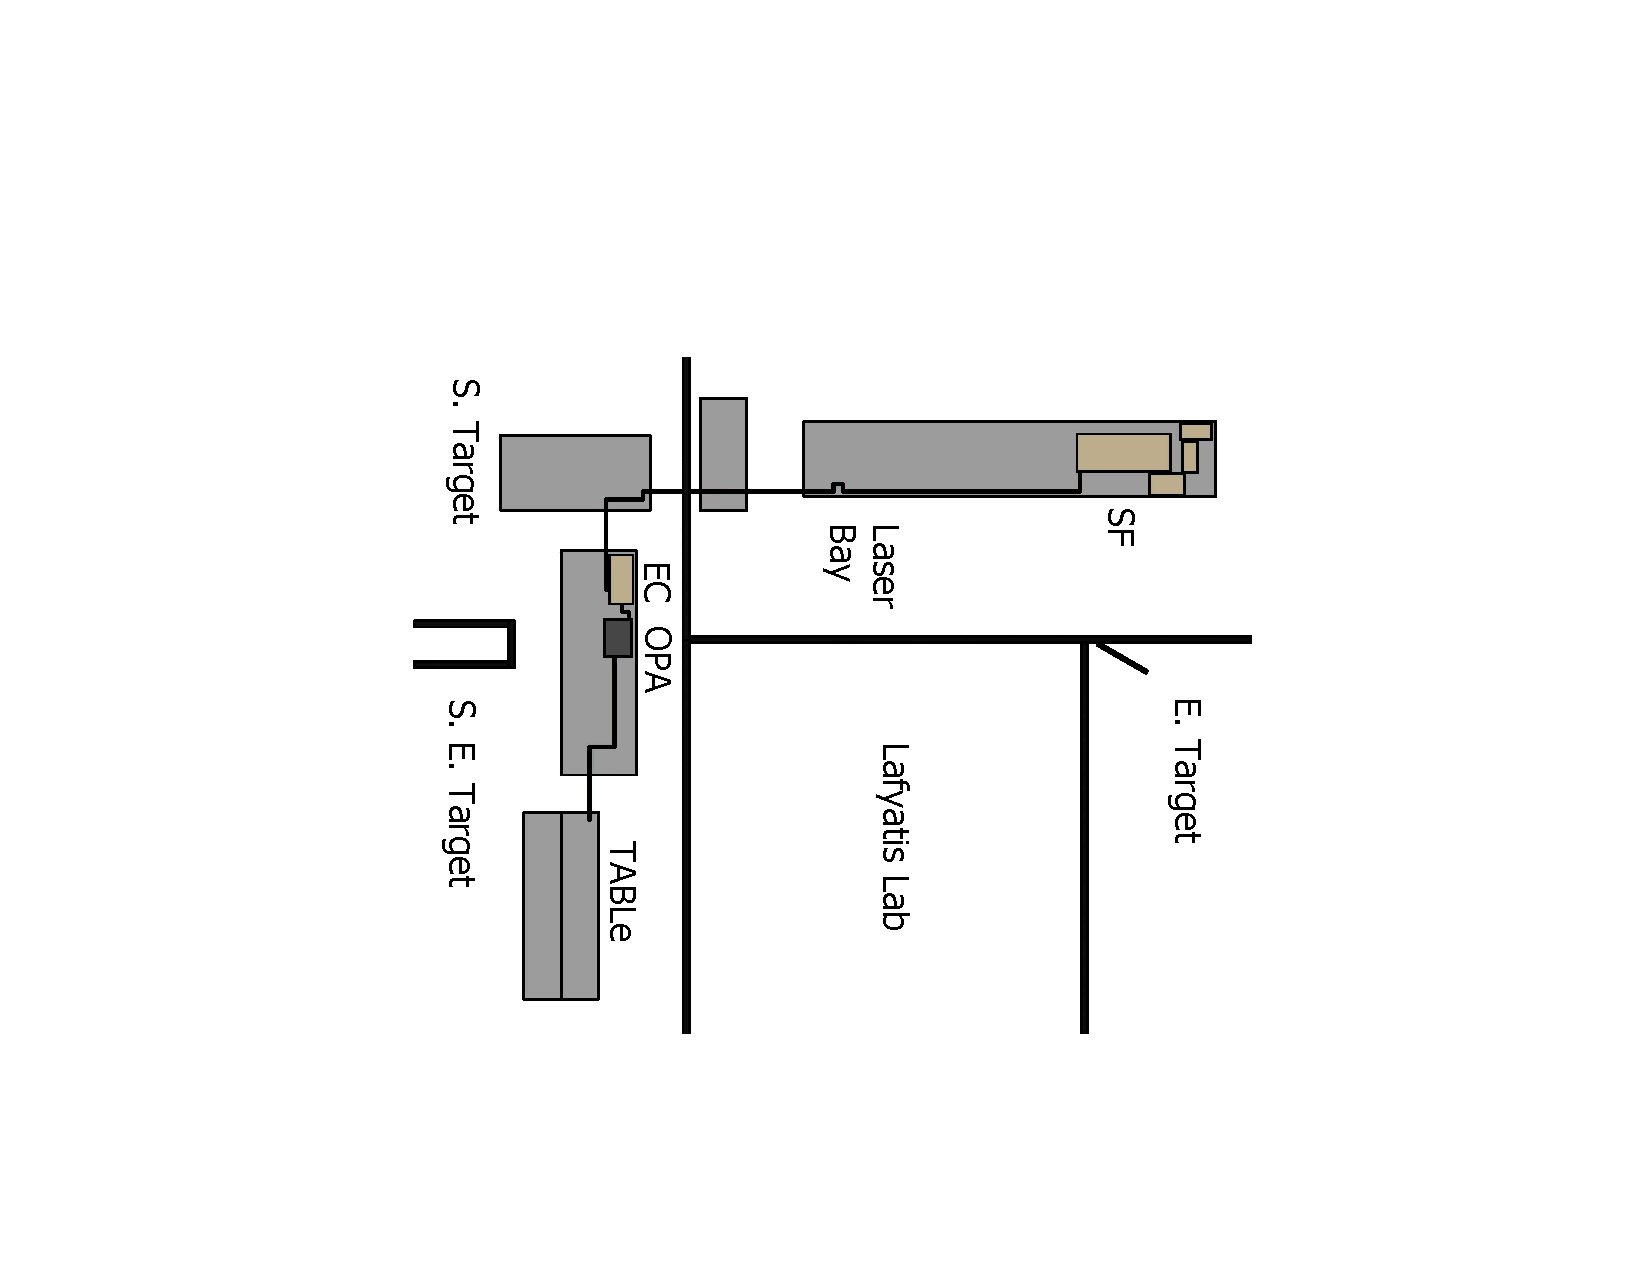
\includegraphics[width=0.95\textwidth,angle=90]{figures/chap2/beam_routing2.pdf}
	\caption{Block diagram of part of the DiMauro lab complex showing the laser path from the laser bay to the southeast target room. Other experiments and laser systems are ommitted for visual clarity. Optical tables are represented as gray boxes. SF: Spitfire laser system consisting of a MaiTai oscillator, two Empower pump lasers, interal stretcher, amplifier \& internal compressor (bypassed for this experiment); EC: Spitfire external compressor; OPA: Light Conversion HE TOPAS Prime; TABLe: $4' \times 10'$ optical table for the transient absorption beamline.}
	\label{fig:beam_routing}
\end{figure}

We use a commercial mid-IR laser system (Spectra Physics Spitfire ACE), which delivers 12 mJ of 800 nm light at a variable $100 - 1,000$ Hz repetition rate with a 60 fs FMHM pulse duration. This system utilizes the chirped pulse amplification (CPA) technique to amplify the pulse energy from a weak seed pulse. In this scheme, a low energy femtosecond seed pulse is stretched in time, amplified and compressed \cite{stricklandCompressionAmplifiedChirped1985}. As such, the Spitfire consists of an oscillator, a grating stretcher, a regenerative amplifier, a single-pass amplifier and a grating compressor.

The laboratory layout is shown in \cref{fig:beam_routing}. All of the lasers in the DiMauro research group are located in a centralized laser bay, where walking traffic is kept to a minimum and air quality is nominally higher than the surrounding laboratory areas. This minimizes air disturbances around the laser systems and reduces the accumulation of dirt and debris on their optics. Experiments are performed in the adjacent target rooms which contain the vacuum systems and other experimental equipment. The Spitfire shares the laser bay with two home-built ultrafast laser systems (the ``2 micron system'' and the ``4 micron system'', not shown in \cref{fig:beam_routing}), as well as some laser development. The Spitfire is positioned so that its light can be directed to either the East, South or Southeast Target Rooms, depending on the needs of the researchers. To reduce air currents, welding curtains surround each optical table in the laser bay. When propagating the beam to target rooms, the beam path is enclosed in PVC tubing to reduce air curtains and to increase user safety. A CaF$_2$ window is used to block air currents between the laser bay and the target rooms.

Referring to \cref{fig:beam_routing}, the transient absorption beamline (TABLe) is located in the southeast target room. Laser light from the amplifier must be propagated uncompressed to the target room to avoid nonlinear propagation effects. To understand why we can compute the $B$ integral, which provides a measure of the nonlinear phase accumulated during propagation: 

\begin{equation}
B = \frac{2 \pi}{\lambda} \int n_2 I(z) \text{ } dz
\label{eqn:B-integral}
\end{equation}
%this calculation was done in B-integral.nb mathematica notebook

The distance between the amplifier and the south target room is approximately 13 meters. For a propagation distance of 13 meters, a beam radius of 0.8 cm, a pulse energy of 12 mJ and a FWHM pulse duration of 60 fs, $B = 1.53$, which indicates that nonlinear propagation effects are significant \cite{zahedpourMeasurementNonlinearRefractive2015}. On the other hand, the uncompressed pulse has slightly higher pulse energy (15 mJ, owing to the 20\% transmission losses of the compressor), but a significantly longer pulse duration ($\sim 10^3$ longer), resulting in a negligible $B$ value. For this reason, we use an external compressor centrally located between the south and south east target rooms, as shown in \cref{fig:beam_routing}. This positioning allows the Spitfire to be used for either the TABLe in the southeast target room or the RABBITT apparatus \cite{chirlaAttosecondPulseGeneration2011,gormanAttosecondProbingElectron2018,kiesewetterDynamicsNearThresholdAttosecond2019} in the south target room (not shown in \cref{fig:beam_routing}). The external compressor has an efficiency of 80\%, giving us 12 mJ of 800 nm light with a FWHM pulse duration of 60 fs at the entrance of the OPA.

The output of the external compressor is sent into a commercial optical parametric amplifier (Light Conversion HE TOPAS Prime), which converts the 800 nm light to longer wavelengths ranging from 1.2 to 2.2 $\mu$m while roughly maintaining pulse duration. To minimize nonlinear propagation effects, the TOPAS is located immediately after the external compressor with only two steering mirrors between the external compressor and the TOPAS. Details of the TOPAS operation, alignment and optimization can be found in the user manual. Briefly, it utilizes a nonlinear process called optical parametric amplification (OPA), where the 800 nm pump ($p$) is converted into two longer wavelength photons (the signal $s$ and the idler $i$) that obey the following energy conservation relation:

\begin{equation}
\frac{1}{\lambda_p} = \frac{1}{\lambda_s} + \frac{1}{\lambda_i}
\end{equation}

Inside the TOPAS, a white light generation process creates a broadband seed pulse, followed by three stages of amplification in BBO crystals. The signal $\lambda_s$ and idler $\lambda_i$ wavelengths are determined by phase matching conditions inside the nonlinear crystals, which is controlled by setting the crystal angle relative to the incident laser light. The BBO crystals are mounted on encoded motorized stages, and the entire system is computer controlled and calibrated so the crystal angles change when the user specifies the desired wavelength. The conversion efficiency of the TOPAS ranges from 40 to 50 \% (combined signal + idler pulse energy of 5 - 6 mJ), depending on the degree of optical alignment into the TOPAS and the desired wavelength. During the amplification process, all three beams are collinear. After the final amplification stage, a dichroic mirror inside the TOPAS separates the depleted 800 nm pump from the signal + idler, and a wavelength separator immediately outside the TOPAS splits the signal from the idler.

\subsection{Active Pointing Correction Systems}

\begin{figure}
	\centering
	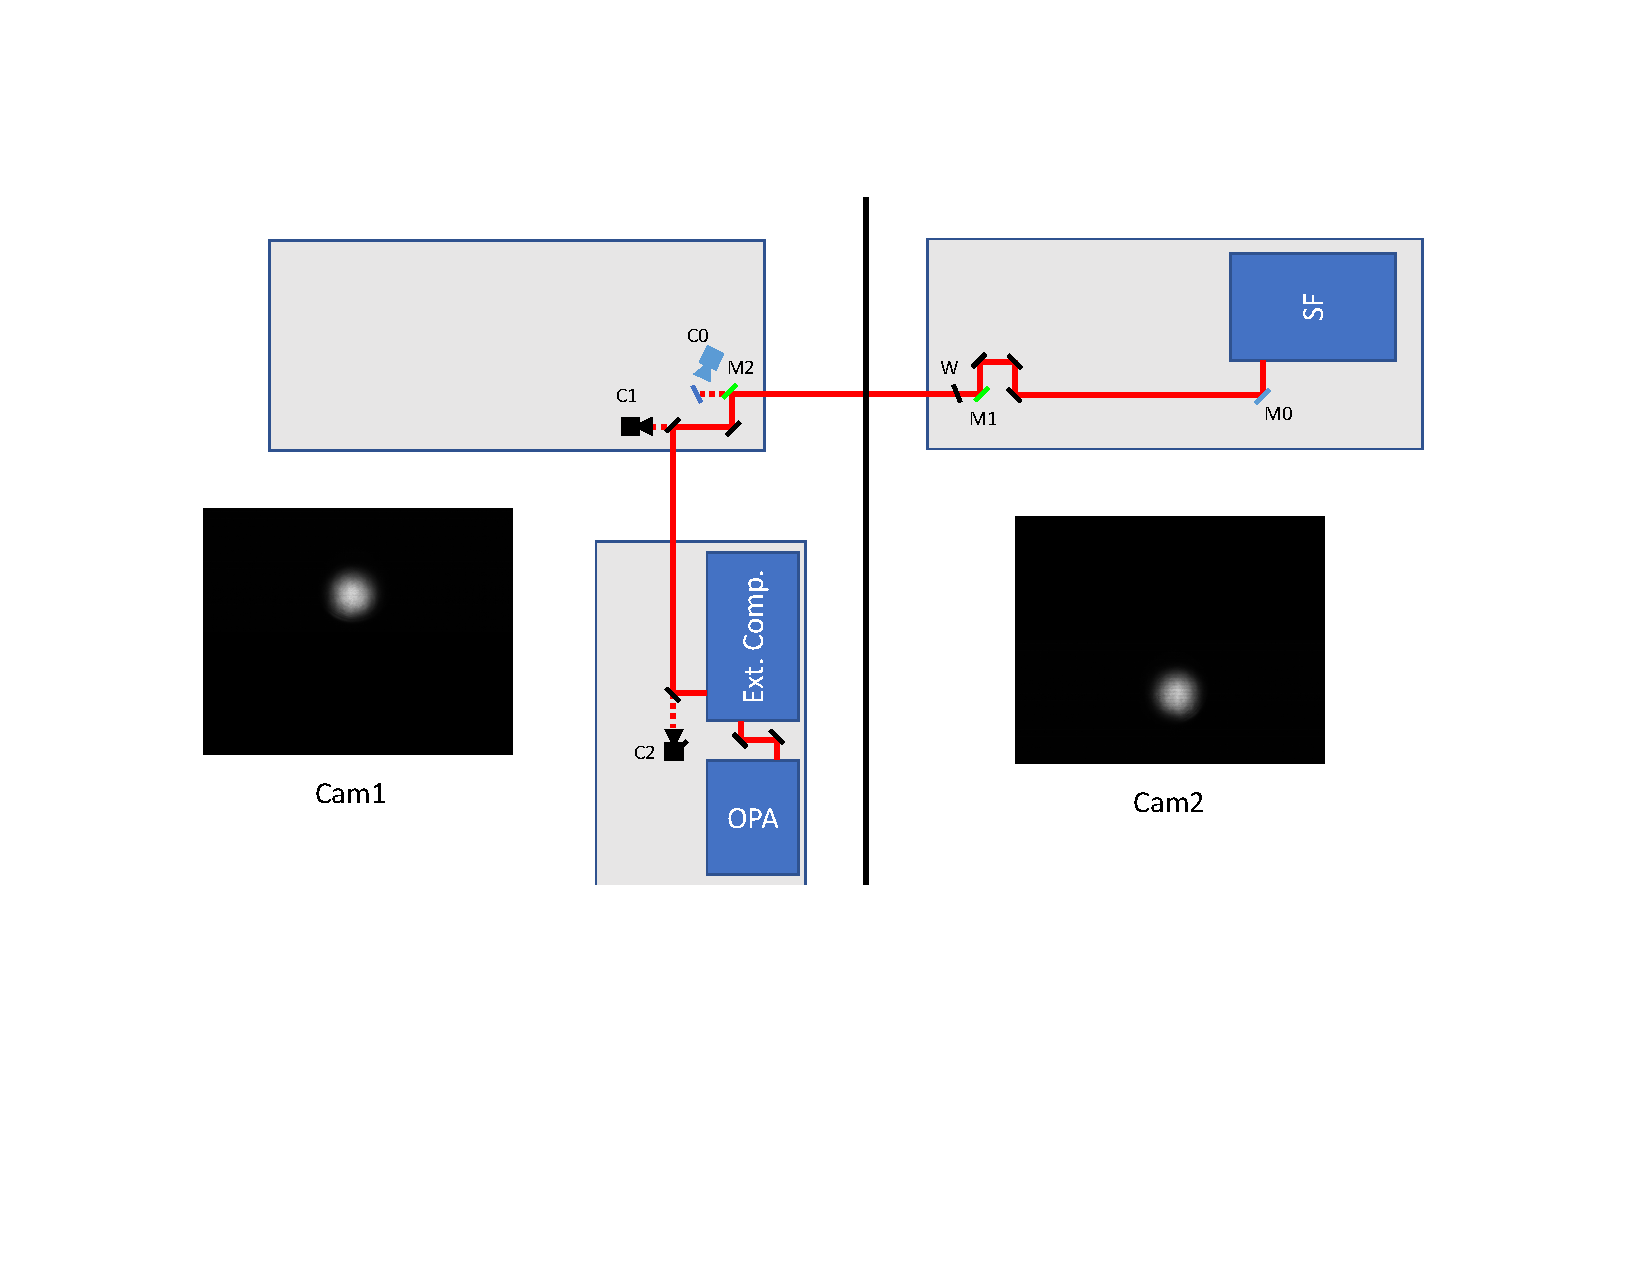
\includegraphics[width=0.75\textwidth]{figures/chap2/guidestar_geometry.pdf}
	\caption{Implementation of active stabilization systems between the amplifier in the laser bay and external compressor in the target room (not to scale). M0 \& C0 are the motorized mirror and digital camera used for the single-point correction scheme. M1, M2, C1 \& C2 are the motorized mirrors and cameras used for the two-point correction scheme. W is an uncoated CaF$_2$ window used to reduce air currents between the laser bay and target rooms. PVC tubes that surround the beam path are omitted for visual clarity. Inset images show the attenuated beam as imaged by C1 \& C2.}
	\label{fig:guidestar_geometry}
\end{figure}

\begin{figure}
	\centering
	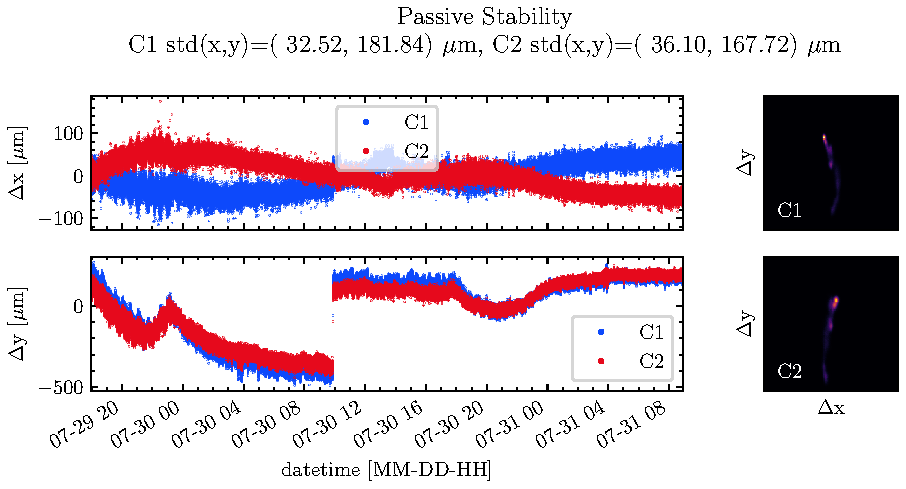
\includegraphics[width=0.75\textwidth]{figures/chap2/Stability_NoCorrection.pdf}
	\caption{Typical passive pointing stability of the Spitfire's amplifier as measured on cameras C1 \& C2. Left panels: $x$ and $y$ coordinates of the centroid vs. time; right panels: 2D histogram of beam centroid positions for the same time period. The 2-point correction scheme was activated between 09:00 (9 am) and 17:00 (5 pm) on 07-30; this system is responsible for the stable performance in the middle in the plot. Long term thermal drift is apparent at all other times.}
	\label{fig:guidestar_passive_stability}
	% dataset: 2019-07-31_8.55am_pointing.txt
	% python file: \Python Scripts\BeamTracker\dissertation_plots.py
\end{figure}

\begin{figure}
	\centering
	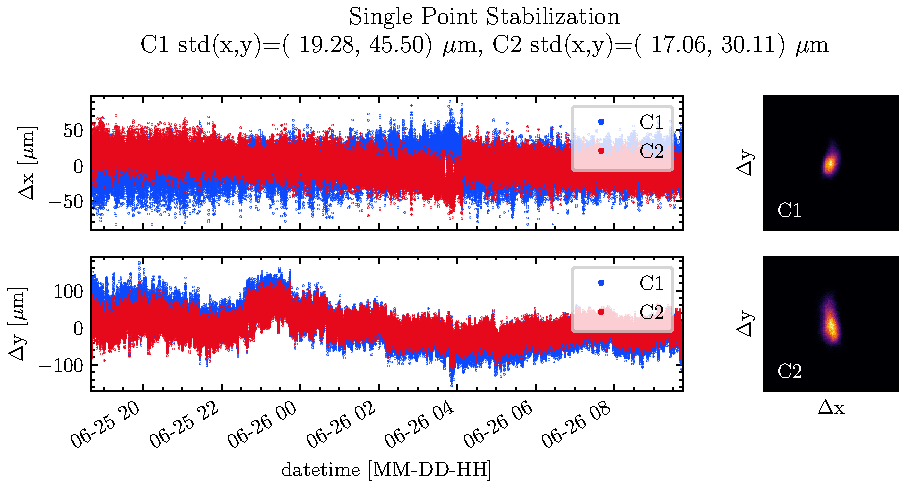
\includegraphics[width=0.75\textwidth]{figures/chap2/Stability_Dietrich_ON.pdf}
	\caption{Single-point stabilization of the Spitfire's amplifier as measured on cameras C1 \& C2. This dataset contains about 10 correction events, which are visible as abrupt jumps in the time series. The skew of the centroid distributions highlights the limitations of the single-point correction scheme.}
	\label{fig:guidestar_1point_stability}
	% dataset: 2019-06-26_09.45am_pointing.txt
	% python file: \Python Scripts\BeamTracker\dissertation_plots.py
\end{figure}

\begin{figure}
	\centering
	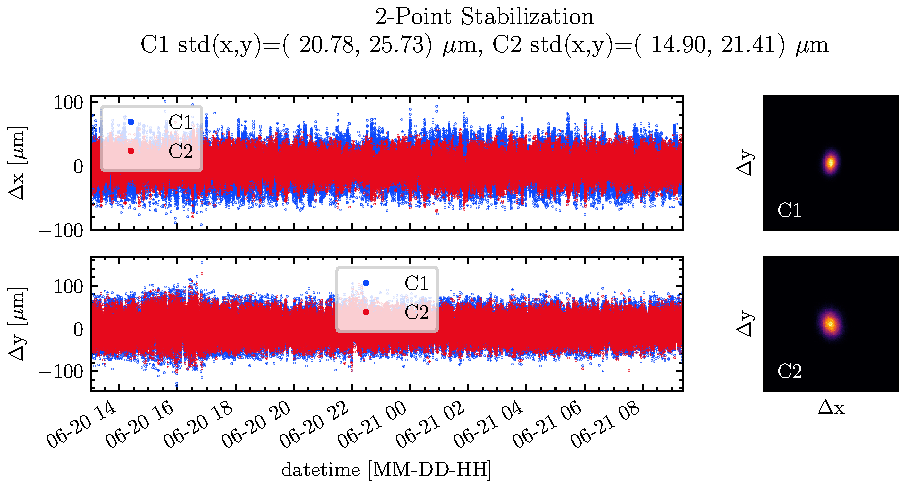
\includegraphics[width=0.75\textwidth]{figures/chap2/Stability_GuideStarII_ON.pdf}
	\caption{Two-point stabilization of the Spitfire's amplifier as measured on cameras C1 \& C2.}
	\label{fig:guidestar_2point_stability}
	% dataset: 2019-06-21_09.23am_pointing.txt
	% python file: \Python Scripts\BeamTracker\dissertation_plots.py
\end{figure}

As a nonlinear device, the performance of the TOPAS is extremely sensitive to input pointing, laser pulse parameters and laboratory environmental conditions. The large optical path length ($\approx 15.5$ m) between the amplifier and the TOPAS puts stringent requirements on the angular tolerances of the amplifier's output pointing. According to the specification sheet, the rms beam pointing stability of the amplifier at constant temperature is $<5\text{ } \mu \text{rad}$ ($\approx 75 \text{ } \mu \text{m}$ at 15.5 m) at constant temperature, which is sufficient for our purposes. Unfortunately, the temperature in the laser bay varies significantly throughout the day -- sometimes by several degrees -- as a function of the occupancy of the physics research building, building-wide energy conservation measures, and activity within the laser bay. Under these conditions, the amplifier's pointing changes by up to 20 $\mu \text{rad} / ^{\circ} \text{C}$ ($= 310 \text{ } \mu \text{m}/ ^{\circ} \text{C}$ at 15.5 m).

To combat this slow pointing drift, we actively stabilize the beam pointing between the amplifier and the external compressor as shown in \cref{fig:guidestar_geometry}. Note that there is not enough space to implement a pointing solution between the external compressor and the TOPAS. Over the years, we have used both a home-built single-point correction scheme and a commercial two-point correction scheme.

\cref{fig:guidestar_passive_stability} shows the passive pointing stability of the amplifier as measured by cameras C1 \& C2 over the course of 28 hours. The left panel shows the $x$ and $y$ coordinates of the centroid (expressed as a deviation from the average position) sampled at 2 Hz. Note that the sign of $\Delta x$ is reversed between C1 and C2; this is an artifact of the camera geometry; otherwise the data from the two cameras is self-consistent. The thermal drift is most apparent in the vertical direction; from midnight to 9 am the beam drifts vertically nearly 500 $\mu$m. Between 9 am and 5 pm we activated the two-point stabilization system (described below), which accounts for the good performance during this time period. At 5 pm, the stabilization system was turned off and the slow drift resumes. The right panels show 2D histograms of the centroid position, calculated from the time series data. From these plots, it is apparent that the laser drifts in a large arc pattern, with the primary deviation occuring in the vertical direction.

The single-point correction system was programmed and implemented by Dietrich Kiesewetter, who was a graduate student at the time \cite{kiesewetterDynamicsNearThresholdAttosecond2019}. In this scheme, a digital camera (C0 in \cref{fig:guidestar_geometry}) located approximately 7.8 m after the amplifier monitors the transmitted light of a high reflective mirror incident on a card. The position of the centroid is calculated on a rolling average basis and compared to a saved set point. When the centroid position deviates from the set point by more than a minimum correction size, a correction signal is sent to a motorized mirror (M0, located 33 cm after the amplifier). The minimum correction size is set by the user to avoid frequent small corrections to the beam, which results in high-frequency pointing jitter. The correction time interval is also user-adjustable, with typical values of 1 - 60 seconds. If the correction signal requires too large of a step, or if the integrated intensity of the beam falls below a set value, then the locking algorithm assumes that something is wrong and breaks the correction loop without taking corrective action. This prevents the system from taking corrective action in the event the beam is partially blocked by a third party.

The performance of the single-point stabilization system as reported by cameras C1 \& C2 is shown in \cref{fig:guidestar_1point_stability}. Here, we can see the limitations of a single-point correction scheme. The system is very good at maintaining the position of the beam at C0, but it has no control over the pointing of the beam. As a result, the beam centroid continues to drift on downstream optics, albeit with reduced magnitude compared to the uncorrected case. This is effect is apparent in the skewed 2D histograms in \cref{fig:guidestar_1point_stability}. The single-point stabilization system works well over short periods of time, but its geometry neccessitates weekly realignment of the external compressor and all other downstream optics. Given the technical demands of our experiments and the sensitivity of the TOPAS to input pointing, this can be a prohibitively time consuming process. Unlike a single-point correction system, a two-point system only needs to be set once.

For the two-point stabilization system, a commercial system was chosen over a home-built solution to reduce the development and implementation time. We use a Newport GuideStar II, which utilizes two cameras (C1 \& C2 in \cref{fig:guidestar_geometry}) and two motorized mirrors (M1 \& M2) to monitor the beam centroid and make corrections. A patented correction algorithm running on purpose-built computational hardware is applied to the output of the cameras to solve for the neccessary correction signals up to 3 times per second \cite{farinasOpticalBeamSteering2009}. Beam pointing is usually recovered with a single corrective action, and even especially large pointing drifts are corrected well within 1 second. For numerical stability and increased sensitivity, the distance between M1 and M2 is made as large as possible (3.1 meters); the distance between C1 and C2 (1.75 meters) is also maximized and made similiar to the M1-M2 distance; the distance between C1 and M2 is made as small as possible (75 cm).

The passive and actively-controlled pointing stability of the amplifier is shown in \cref{fig:guidestar_2point_stability}. Owing to the high correction frequency, individual corrections are small and not visible in the time series. The two-point system maintains both the centroid position and propagation direction, so there is minimal correlation between the reported centroid positions on C1 \& C2. As a result, the pointing into the TOPAS rarely needs to be optimized under normal operation, saving valuable time and making experiments more repeatable.

The GuideStar II performs extremely well, but its software lacks the safety features of our home-built system. Specifically, there is no maximum allowable correction size, intensity or beam mode quality monitoring to prevent run-away corrections. For example, it is common to insert a paper card into the beam path to inspect the beam mode just before the external compressor. As a result, camera C2 will briefly see a partially clipped beam with a centroid displaced by approximately the beam radius, and the GuideStar will take \textit{immediate corrective actions} to adjust the pointing. These actions may result in a 15 mJ beam pointing in an unsafe direction. \textbf{Users are cautioned to keep clear of the beam path between the amplifier and the GuideStar cameras when the GuideStar locking algorithm is enabled.} To mitigate this issue, the GuideStar cameras are kept in a plastic enclosure and workers are made aware of the limitations of the GuideStar system.

\textbf{say something about the 2photon photodiode in the external compressor}

\subsection{Beam routing into the TABLe interferometer}

After selecting the wavelength (signal, idler or depleted pump), the output of the TOPAS is sent approximately 3 meters downsteam to the transient absorption optical table. Two motorized mirrors on the TOPAS optical table are used to align the laser into the TABLe interferometer. Unless otherwise noted, protected silver mirrors are used to propagate the TOPAS light for their broadband reflectivity, low absorption losses and high corrosion resistance. 

\section{Vacuum System}
\label{sec:Vacuum_System}
\subsection{The Need for High Vacuum}

\begin{figure}
	\centering
	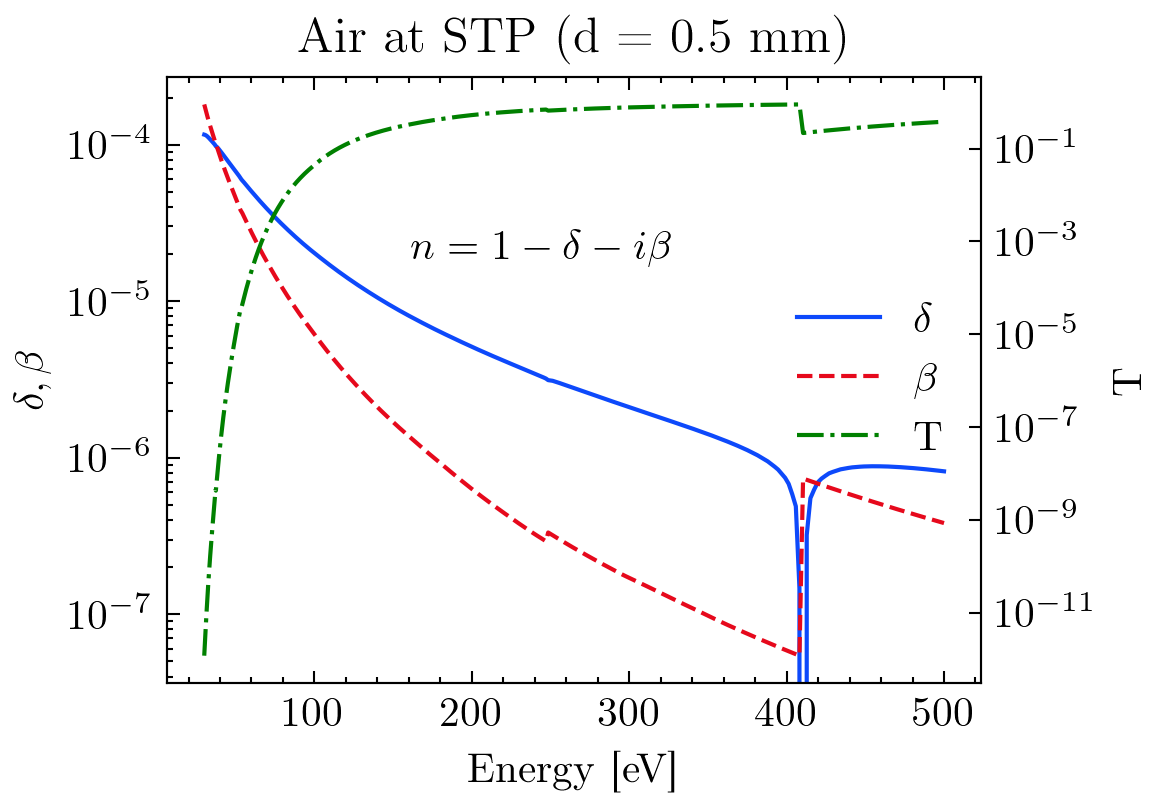
\includegraphics[width=0.75\textwidth]{figures/chap2/AirAbs.png}
	\caption{Estimation of XUV propagation losses through 0.5 mm of air at STP. Atomic scattering data obtained from \cite{gulliksonCXROXRayInteractions,henkeXRayInteractionsPhotoabsorption1993}. Calculation follows \cref{eqn:PhotoCrossSection,eqn:BeersLaw,eqn:IndexfromASF}.}
	\label{fig:AirAbs}
	% generated using CXRO.py
\end{figure}

\begin{figure}
	\centering
	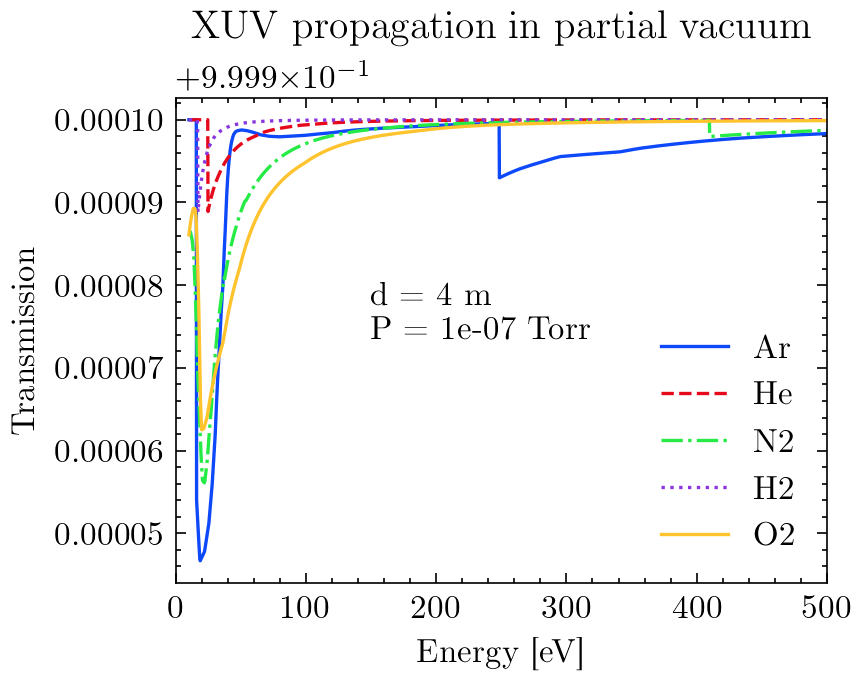
\includegraphics[width=0.75\textwidth]{figures/chap2/XUVinVacuum.png}
	\caption{Estimation of XUV propagation losses through a vacuum level of $10^{-7}$ Torr and a distance of 4 meters. Transmission is well over 99.99\% for this pressure-length product. Atomic scattering data obtained from \cite{gulliksonCXROXRayInteractions,henkeXRayInteractionsPhotoabsorption1993}. Calculation follows \cref{eqn:PhotoCrossSection,eqn:BeersLaw,eqn:IndexfromASF}.}
	\label{fig:XUVinVacuum}
	% generated using CXRO.py
\end{figure}

The XUV light generated by the high harmonic process is absorbed strongly by air, as most gases have at least one electronic transition in the XUV regime. The magnitude of absorption can be estimated using the atomic scattering factors $f = f_1 + i f_2$, which were taken from \cite{henkeXRayInteractionsPhotoabsorption1993}. The photoabsorption cross section $\mu_a$, the transmission ratio $T$, and the complex index of refraction $\hat{n}$ of a gas can be calculated from these factors:

\begin{equation}
\mu_a = 2 r_0 \lambda f_2
\label{eqn:PhotoCrossSection}
\end{equation}

\begin{equation}
T = \exp\left( -N \mu_a d \right)
\label{eqn:BeersLaw}
\end{equation}

\begin{equation}
\hat{n} = 1 - \frac{1}{2 \pi} N r_0 \lambda^2 \left(f_1 + i f_2\right)
\label{eqn:IndexfromASF}
\end{equation}

In the above equations, $\lambda$ is the photon wavelength, $N$ is the number of atoms per unit volume, $d$ is the optical path length and $r_0=2.8179403227(19) \times 10^{-6} \text{ nm}$ is the classical electron radius. The results for air at standard temperature and pressure are shown in \cref{fig:AirAbs}. From this figure it is apparent that any XUV light we generate will be effectively attenuated to zero in less than 1 millimeter if the beam is propagated in air.

For reference, the XUV portion of the transient absorption beamline is about 4 meters long. \cref{fig:XUVinVacuum} shows the expected XUV transmission losses for XUV propagation through a partial vacuum of common gases: argon and helium are often used for generation, while nitrogen, hydrogen and oxygen are common UHV system contaminants. From this figure, we can see that the XUV transmission exceeds 99.99\% for an average pressure of $10^{-7}$ Torr. Note that this calculation does not include reflection losses from the ellipsoidal mirror, transmission losses from the metallic filter or the sample, or geometric losses from clipping. This simple analysis tells us that the XUV portion of the beamline must be kept under relatively high vacuum to avoid needlessly reducing the XUV flux.

The microchannel plate (MCP) assembly in the photon spectrometer (see \cref{sec:XUV_spectrometer}) puts additional constraints on the vacuum level.  Contaminants in the spectrometer chamber (originating from a finite chamber pressure) lower the effective electrical resistance between the highly charged plates, resulting in a somewhat periodic current surge between the plates. This effect manifests itself in the data as a bright point source at a random location on the detector. In addition to reducing the fidelity of the data, each current surge counts towards the lifetime limit of the MCP assembly, reducing its lifetime \cite{ladislaswizaMicrochannelPlateDetectors1979}.

The low pressure condition required to minimize XUV absorption and instrumentation malfunction is in direct conflict with the requirements for high harmonic generation (HHG) and gas-phase attosecond transient absorption spectroscopy (ATAS) experiments. HHG requires a gas source to be placed near the IR focus in the generation chamber, and a gas-phase ATAS experiment requires a similar gas source to be placed near the XUV/IR focus in the target chamber. The gas from these sources will diffuse into neighboring chambers, raising the pressure of the entire beamline. In addition to the complications described above, higher pressures can overwhelm and damage the turbomolecular vacuum pumps used to keep the system at high vacuum. The vacuum apparatus was designed to localize the gas density at the interaction regions while allowing a range of optical configurations to be used.

\subsection{Design Goals}

The vacuum system was designed to be as modular as possible. In this sense, the TABLe apparatus can be thought of a permanently installed XUV light source \& XUV-IR interferometer that has the ability to accept modular end stations. This design priniciple has already allowed the study of electron rescattering in strong infrared fields by another graduate student \cite{kiesewetterDynamicsNearThresholdAttosecond2019}; going forward, new target chambers can be designed to meet the needs of future experiments while maintaining the integrity of the XUV light source and interferometer.

We employ magnetically levitated turbomolecular pumps which were not commercially available at the time of the RABBITT apparatus' construction. These pumps are designed so that the vacuum side of the blade assembly does not make mechanical contact with the drive shaft and housing, which dramatically reduces vibrations during operation. Mag-lev turbopumps have a noise power spectrum an order of magnitude smaller than that of traditional turbopumps. This ultra-quiet operation allows us to mount the vacuum hardware directly on the interferometer's optical table. Likewise, we keep our rough vacuum system in an adacent pump room to minimize acoustics, vibrations and oil contamination in the target rooms.

Large vacuum chambers have the benefit of being able to accommodate a seemingly limitless amount of optics and internal hardware, but they are very uncomfortable and difficult to work around. For this reason, we tried to keep the physical size of the chambers as small as possible while still allowing sufficient internal space for our current and reasonable future equipment needs (\textit{in vacuo} motorized stages, optics, gas and electric feedthroughs, etc.). Additionally, \textit{in vacuo} optics are difficult to optimize. Vacuum compatible optic mounts exist, but they are expensive, cumbersome to work with and generally considered specialty items that need to be custom ordered. Adjusting a non-motorized optic requires a venting / pumping cycle, which can take several hours. Early on in the design process, we made the decision to keep as many optics as possible outside of the vacuum system, greatly reducing the overall size of the system. Excluding the modular endstations, our vacuum chambers have a footprint that is approximately one third that of the RABBITT apparatus, which leaves more than half of our $4' \times 10'$ optical table unoccupied.

\subsection{Manufacturing Considerations}

When we started this project, the DiMauro lab already had a working attosecond beamline: the RABBITT apparatus, located in the south target room \cite{chirlaAttosecondPulseGeneration2011}. We considered modifying this apparatus for our needs, but ultimately decided to build a second beamline. The RABBITT apparatus was being frequently used by more senior students working on projects with experimental requirements that were in conflict with those of a transient absorption experiment \cite{kiesewetterDynamicsNearThresholdAttosecond2019,gormanAttosecondProbingElectron2018}. At the minimum, we needed to build an XUV photon spectrometer and a condensed matter sample holder. We could have removed the electron spectrometer from the RABBITT apparatus and installed a condensed matter target chamber and photon spectrometer, but this would have been extremely disruptive to the rest of the group. Furthermore, the south target room was already crowded with the cluster apparatus \cite{wangMidinfraredStrongfieldLaser2018}, and our equipment would not fit in the room without significant modification to the existing laboratory environment. Also around the start of this project, the DiMauro lab complex was expanded by half a standard laboratory unit (one half of PRB 4115). A partial wall (about 12 feet high) was constructed in 4115, separating the Lafyatis lab from what would now be called the south east target room. Next, the wall separating the south and our half of 4115 was knocked down. The current lab layout can be seen in \cref{fig:beam_routing}.

Modular aluminum vacuum chambers were not yet available on the commercial market \cite{piperAndrewPiperDissertation}, so we went with a welded design for our custom chambers. We considered both aluminum and stainless steel (SS) for the chamber material. Aluminum was preferred for our application, as it is lighter and therefore easier to mount to an optical table. Due to the presence of a natural oxide layer, aluminum chambers have difficulty reaching UHV vacuum; fortunately our experimental requirement of $10^{-7}$ Torr is well within reach of an aluminum chamber. The biggest concern of an all-aluminum chamber was the softness of an aluminum knife edge. Recalling the geometry of a conflat flange, the ``knife edge" is used to form a semi-permanent metal-metal sealing surface between the conflat and a metal gasket. Any imperfections in the knife edge will result in a sub-optimal sealing surface and will leak. The concern was that an aluminum knife edge could be easily damaged while working in and around the chamber. The solution to this problem is to use SS conflats with an Al chamber body. However, Al and SS cannot be welded together using traditional welding techniques; they must be joined using a difficult technique called \textit{explosive welding}. Few companies are able to explosively weld UHV chambers, and those that do charge a premium for their manufacturing services. A mixed-metal chamber would have been prohibitively expensive, so we decided to use an all stainless steel design.

We decided to have our custom chambers manufactured by the Physics and Astronomy Machine Shops. This allowed us to consult with the machinists frequently during the design phase, which allowed us to converge on a design that met our experimental requirements while minimized machining operations and cost. To this end, we used off-the-shelf vacuum hardware (standard vacuum crosses, full nipples, etc.) whenever possible. The physical size of the ellipsoidal mirror and the XUV spectrometer neccessitated a custom chamber design. To minimize engineering and machining complexity, we designed these chambers as simple ``boxes", i.e., using plate geometry.

%The DiMauro group has extensive experience working with home-built vacuum hardware and attosecond interferometry. At the beginning of this project, we drew heavily on the expertise of group members when designing our vacuum system. Because the technical requirements of our vacuum system are very similar to that of the RABBITT apparatus \cite{chirlaAttosecondPulseGeneration2011}, we will frequently make comparisons between the two devices. An overview of the TABLe's vacuum system can be seen in \cref{fig:TABLE_overhead_drawing,fig:TABLE_angled_drawing}.


\subsection{Vacuum System Details}

\begin{sidewaysfigure}
	\centering
	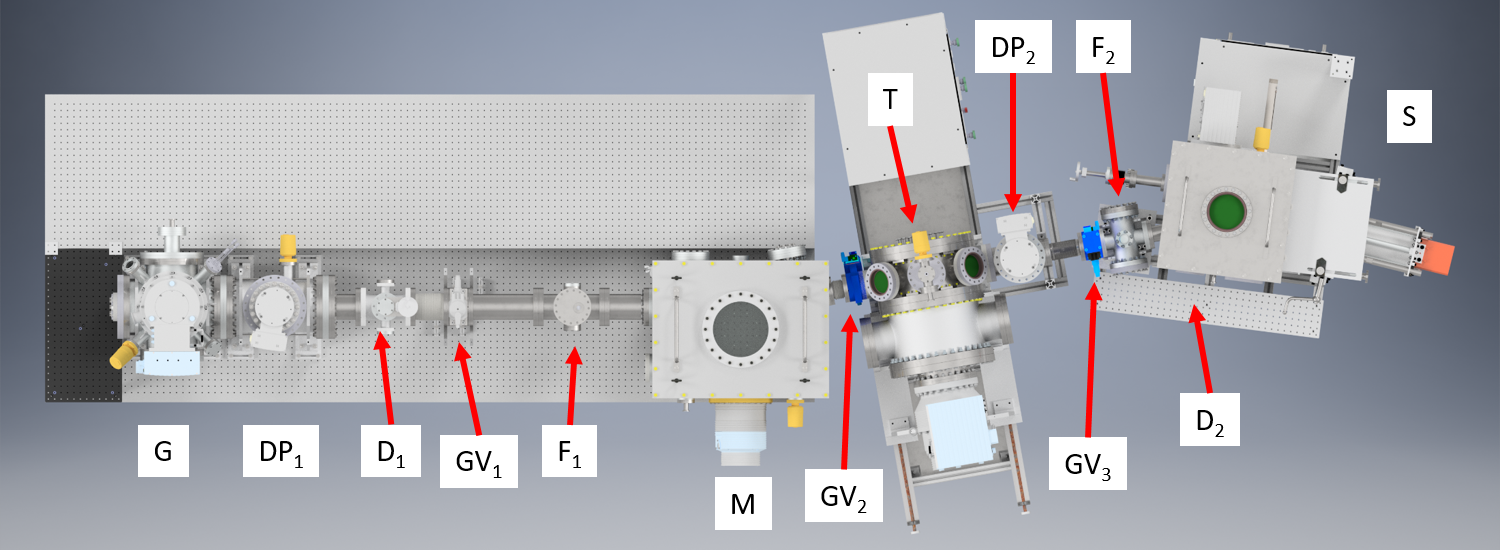
\includegraphics[width=1.0\textwidth]{figures/chap2/TABLe assembly - overhead labeled.png}
	\caption{Overhead rendering of the TABLe's vacuum chambers. In-air optics are omitted for visual clarity. G: generation chamber; DP: differential pumping chamber; D: IR diagnostic station; GV: gate valve, F: metal filter; M: mirror chamber; T: target chamber; S: XUV photon spectrometer.}
	\label{fig:TABLE_overhead_drawing}
	%  rendered using Inventor Studio (png). labels added in powerpoint
\end{sidewaysfigure}

\begin{sidewaysfigure}
	\centering
	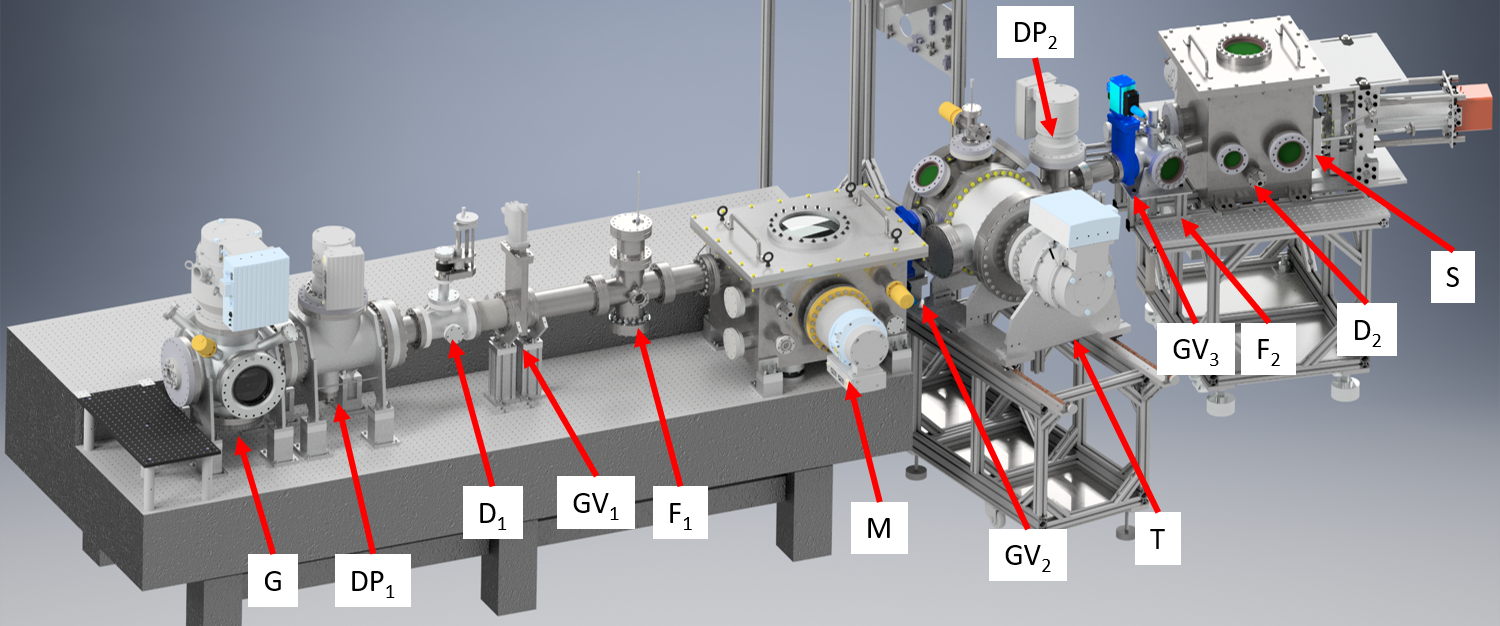
\includegraphics[width=1.0\textwidth]{figures/chap2/TABLe assembly - angled labeled.png}
	\caption{Angled rendering view of the TABLe's vacuum chambers showing the two-level 4' $\times$ 10' optical table. G: generation chamber; DP: differential pumping chamber; D: IR diagnostic station; GV: gate valve, F: metal filter; M: mirror chamber; T: target chamber; S: XUV photon spectrometer.}
	\label{fig:TABLE_angled_drawing}
	%  rendered using Inventor Studio (png). labels added in powerpoint
\end{sidewaysfigure}


In this section, we will provide a brief overview of each vacuum chamber in the TABLe vacuum system. A render of the final vacuum design is shown in \cref{fig:TABLE_overhead_drawing,fig:TABLE_angled_drawing}. A cartoon of the beam path showing the beam path relative to the vacuum system is shown in \cref{fig:beamline_schematic}.

The first half of the vacuum system sits atop a custom split-level 4' $\times$ 10' optical table (TMC Vibration Control). The lower deck of the table is 24" wide and 12" thick and the upper deck is 20" thick. With this design, we are able to place the vacuum chambers directly on the lower deck while keeping the beam height of the in-air components at a standard height above the upper deck of the table. Like all other optical tables in the DiMauro lab, this table is not pneumatically floated; it sits directly on a steel leg assembly. This maintains the relative position between the optical tables and allows us to put the weight of the chambers on top of the table.

The second half of the vacuum system is not directly connected to the optical table, but instead sits on floor-mounted extruded aluminum frames. This modularity allows us to swap the endstations as dictated by experimental requirements. Although this makes these chambers less mechanically stable, this is an acceptable compromise as they are not part of the interferometer.

We use three gate valves to create four different vacuum regions in the beamline. This allows us to vent or pump down these sections independently, which is useful when trying to preserve air-sensitive components (MCP, metal filters, samples) or to minimize downtime when performing a ``quick fix" that neccessitates venting a single section. All three gate valves are electro-pneumatically powered so that they can be controlled via the OMRON safety system. GV$_1$ it is positioned between the IR diagnostic station and the metal filter, upstream of the ellipsoidal mirror. GV$_2$ is located between the mirror and target chambers. GV$_3$ is located between the target chamber's differential pump and the spectrometer's filter chamber. The four vacuum sections are colloquially referred to as the generation chamber, the mirror chamber, the target chamber and the spectrometer.

Pressures in each chamber are monitored using a combination Pirahni / cold cathode pressure gauge (Leybold PTR90) that can read pressures from 750 Torr to $7.5 \times 10^{-9}$ Torr. Each vacuum section has a CF-to-KF adapter fitted with a blank KF flange, which is loosened while venting to prevent overpressurization of each vacuum section. The pressure in each turbo pump foreline is monitored by a thermocouple pressure gauge (Lesker KJL-6000) and analog controller.

\subsubsection{Generation and Differential Pump Chambers}

The first chamber in the vacuum system is the \textit{generation chamber} (G), where the XUV light is produced via HHG. Attached to this chamber and separated by a vacuum aperture is the \textit{differential pumping chamber} (DP$_1$). The geoemtry of these two chambers localizes the high gas pressures required for HHG within the generation chamber.

The generation chamber is designed to house the HHG gas nozzle or cell, and short focal length optics. It is here that the XUV light is created for the ATAS experiments. As such, it must be large enough to house an XYZ translation stage, as well as the neccessary electric and gas line feedthroughs. The turbo pump must be large enough to maintain milliTorr or lower pressures while being subjected to large gas throughputs for the duration of an experiment. The geometry of the chamber must accommodate a range of focal lengths and optical layouts. To facilitate IR/gas nozzle alignment, there must be a clear line of sight from outside the chamber to the IR's focal spot (roughly, the center of the generation chamber).

The generation chamber is a standard 6-way 10" ConFlat (CF) cross that has been modified by the Physics Machine Shop to have four additional 2.5" CF ports. These so-called \textit{radial ports} are positioned at the corners of the top flange and are directed towards the center of the generation chamber. The 10" CF flanges are populated as follows. A large turbo pump (Oerlikon Leybold Turbovac Mag W 1300 iP, 1300 Liter/sec) is mounted on the top 10" CF flange. The bottom flange has a 50-pin electric feedthrough and tapped holes for mounting an internal aluminum breadboard, which holds the motorized XYZ manipulation stage, gas nozzle / cell, and any focusing optics. The front flange has zero length adapter with a custom o-ring sealed optical window mount (2" diameter, 1.5" clear aperture, 3 mm thick CaF$_2$), which lets the laser light enter the chamber. A large 8" diameter viewport is mounted on the right flange, and a CF-to-KF adapting flange for the HPC (see \cref{sec:HPC}) is mounted on the left flange. The rear flange holds the vacuum aperture assembly and a double-sided 10" CF flange, which connects to the front flange of the differential pump chamber. The 2.75" radial flanges hold a Leybold pressure gauge, a 2" diameter viewport and a 4-pipe 1/8" Swagelok gas feedthrough flange (Lesker).

The vacuum aperture assembly is modular, as it allows different sized apertures to be installed as neccessary. Currently, we use a 10 mm diameter aperture which was chosen to maximize the XUV transmission downstream. This setup yields a pressure drop of about 2 orders of magnitude across the aperture.

The differential pumping chamber is a standard 3-way 10" CF tee with two additional 2.75" CF flanges pointing towards the optical axis. The front 10" CF flange is connected to the generation chamber; the top CF 10" flange holds a small turbo pump (Oerlikon Leybold Turbovac Mag W 400 iP, 400 L/s) and the rear 10" CF flange connects to the IR diagnostic station. A KF blow-off assembly and a pressure gauge are mounted to the 2.75" CF flanges.

The turbo pumps for these two chambers are backed by rotary vane (RV, Leybold D65B, 65 m$^3$/hr) and roots blower (Leybold WSU 501, 500 m$^3$/hr) pump stack located in an adjacent pump room. This rough vacuum system is connected to the beamline via a large diameter copper and PVC tube. The pressure at the inlet flange of the roots blower is remotely monitored using an thermocouple gauge (Agilent Type 0531 TC) an electronic gauge controller (Lesker KJL615TC-E), a wireless networking router, and a touchscreen-enabled Raspberry Pi running Lesker's web applet.

Typical operating pressures using a 200 $\mu$m diameter free expansion nozzle (Argon gas, $P_0 = -5$ psig backing pressure, 2.75 Torr-liter/second throughput) are about 3 mTorr in the generation chamber and $5 \times 10^{-5}$ Torr in the differential pump chamber.

\subsubsection{IR Diagnostic Station}

An \textit{IR diagnostic station} (D$_1$) is located after the differential pumping chamber. The diagnostic station houses a silver mirror mounted to a linear shift mechanism. When retracted, the mirror is out of the optical axis; when inserted the IR beam is diverted outside of the vacuum system through a window onto the upper deck of the split level optical table. This diagnostic station is used to measure the transmitted power of the generation arm when aligning the high pressure cell (HPC, see \cref{sec:HPC}).

\subsubsection{Filter Chamber}

\begin{figure}
	\centering
	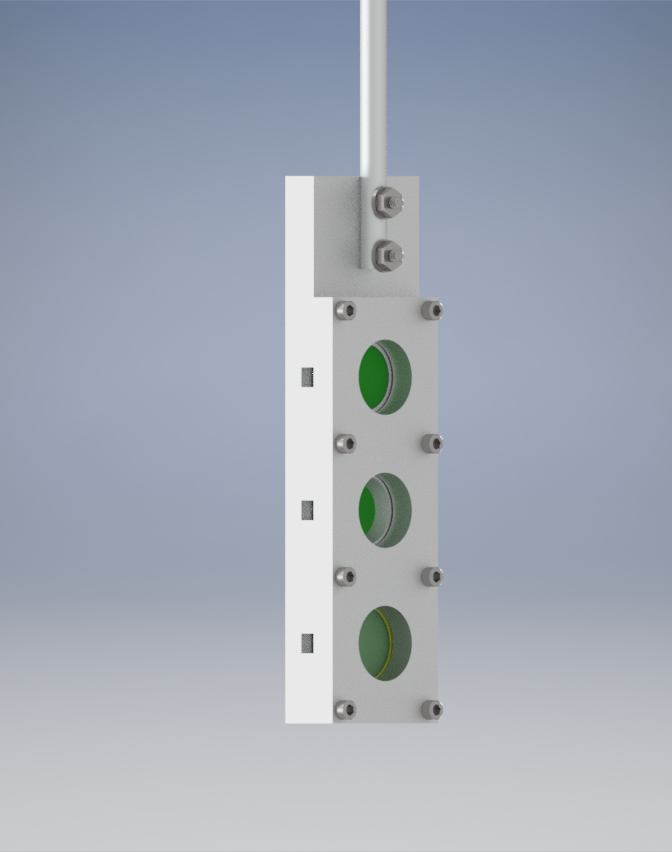
\includegraphics[width=0.50\textwidth]{figures/chap2/filter_stick.png}
	\caption{Rendering of the metallic filter assembly in the spectral filter chamber. Metallic filters are shown with a false green color for visual clarity.}
	\label{fig:filter_stick}
	% generated using Inventor Studio
\end{figure}

The generation arm's IR light is blocked at the first spectral \textit{filter chamber} F$_1$, which is located after the diagnostic station and before the XUV mirror. This chamber houses a o-ring sealed insertable rod upon which a clamshell assembly is mounted, as shown in \cref{fig:filter_stick}. This assembly was designed to hold standard metallic filters made by Luxel or Lebow, or achromatic MCP filters \cite{zhangSuppressionDrivingLaser2014}. By changing the insertion of the rod into the chamber, the user can select which of the three filters is on the optical axis. A calibrated indicator located outside the chamber (not shown) has markings to indicate the approximate rod position for each filter. The precise height of the filter can be fine tuned while observing the spatial profile of the XUV beam, as reported by the XUV spectrometer. Note that using a mesh-supported filter will imprint a grid-like pattern into the XUV beam, which will be apparent in the spectrometer's readings. Retracting the rod fully allows the XUV-IR beam to continue down the beamline unattenuated. Users should are cautioned that the IR light in an unfiltered beam will destroy condensed matter samples in the target chamber.

\subsubsection{Mirror Chamber}

\begin{figure}
	\centering
	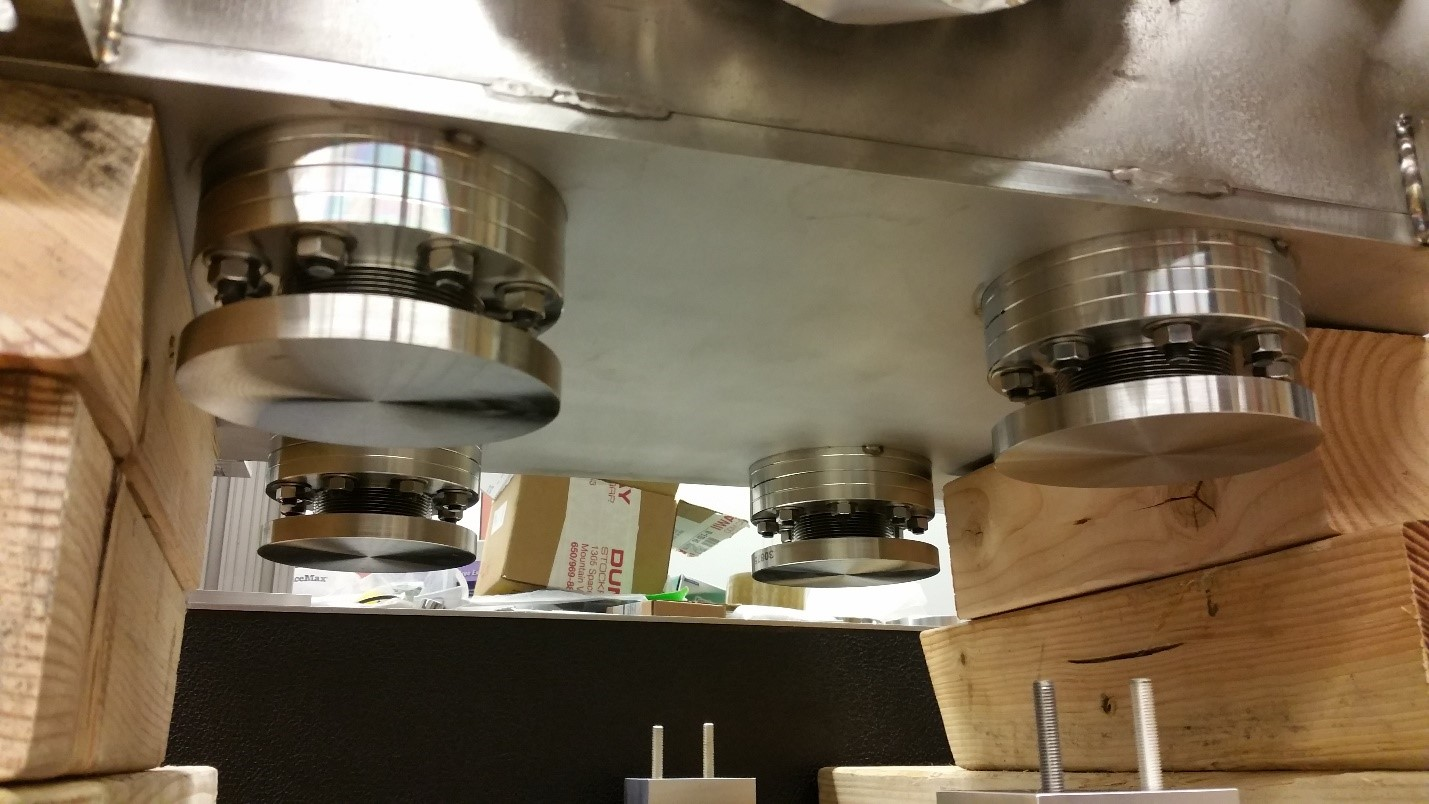
\includegraphics[width=0.75\textwidth]{figures/chap2/mirror_chamber-bellows_feet_lowres.jpg}
	\caption{Photograph of the underside of the mirror chamber showing the vibration-dampening bellows during installation. Steel rods (not visible) connect the interior of the bellows feet to the interior breadboard. After installation, the flat metal disks were secured to the optical table using clamps.}
	\label{fig:mirror_chamber_bellows_feet}
	% generated using Avant.CAD screenshot tool
\end{figure}

\begin{figure}
	\centering
	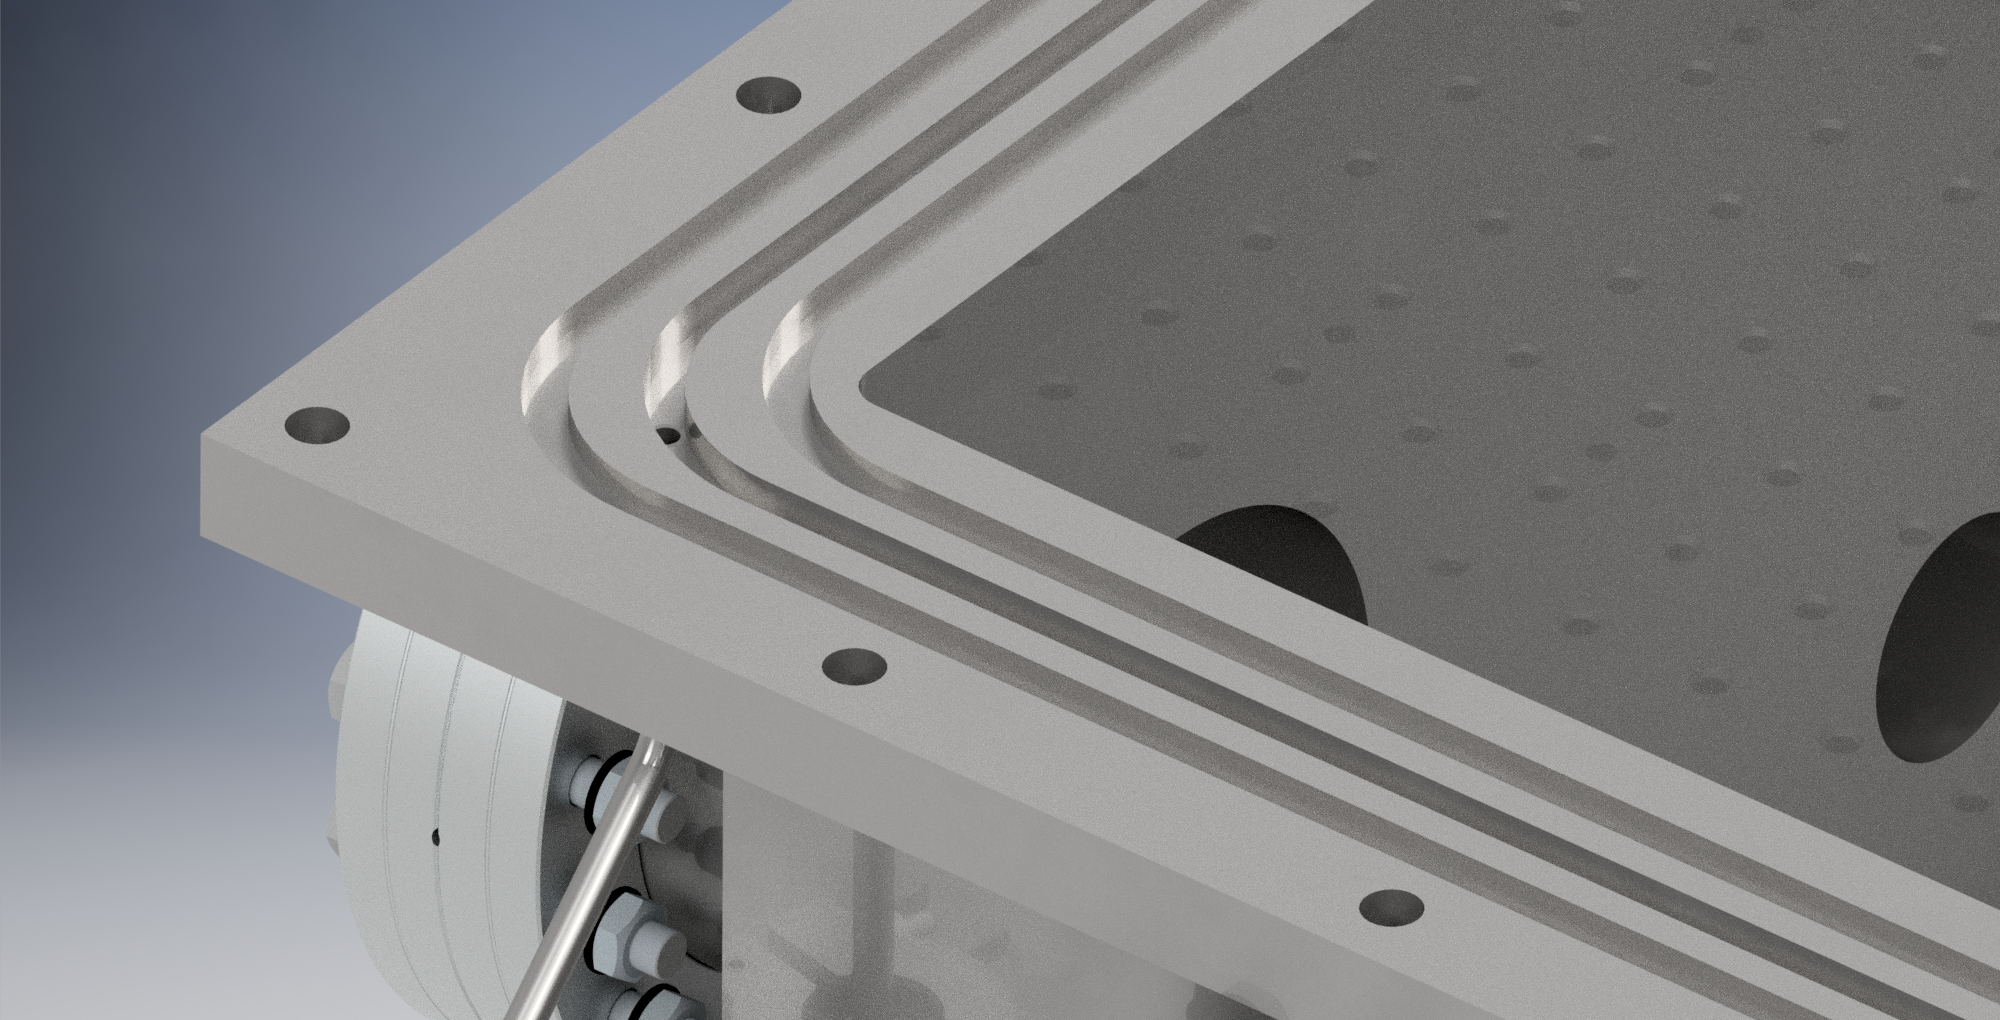
\includegraphics[width=0.75\textwidth]{figures/chap2/mirror_chamber-diff_pump_groove.png}
	\caption{Rendering of the mirror chamber's sealing surface showing detail of the differentially pumped double o-ring. O-rings are not shown in this figure. The two o-ring glands, the central pumping channel and the welded 1/4" stainless steel pumping tube are visible. Four through holes for the 5/16" sealing bolts are visible at the perimeter of the chamber's sealing surface.}
	\label{fig:mirror_chamber_diff_pump_groove}
	% generated using Avant.CAD screenshot tool
\end{figure}

The \textit{mirror chamber} (M) is located after the filter chamber at the end of the 4' $\times$ 10' optical table. This chamber houses the ellipsoidal and hole mirrors (discussed in \cref{sec:Interferometer_Design}). The ellipsoidal mirror (EM) reimages the XUV source onto the target, while the hole mirror (HM) collinearly combines the generation arm's XUV with the pump arm's IR, closing the interferometer. The two pulses leave the chamber through the exit flange, which is angled 10 degrees to the left to account for the 85 degree incident angle of the EM.

This chamber has windowed ports (2 inch diameter, 3 mm thickness CaF$_2$) that allow for positioning of the hole mirror before or after the ellipsoidal mirror, depending on experimental requirements. If the EM precedes the HM, then the IR pump arm focal parameters can be tuned arbitrarily, but this flexibility comes at the cost of having an additional optic in the interferometer. If the HM precedes the EM, then both the XUV and the IR pump share a common focusing optic which is outside the interferometer, which can improve interferometric stability.

An internal reinforced aluminum breadboard supports the optomechanical components within the chamber. This breadboard is mechanically coupled directly to the 4' $\times$ 10' optical table using four stainless steel columns that run through openings on the underside of the mirror chamber, as shown in \cref{fig:mirror_chamber_bellows_feet}. Each port has a soft bellows housing that isolates chamber vibrations (originating from the pumping system) from the interferometrically stable optics within the chamber. 

It is important to have remote \textit{in vacuo} control of both the EM and the HM, as the final alignment must be done with the XUV light. The optomechanical support of the ellipsoidal mirror was designed to avoid the cantilevering present in the XUV mirror of the RABBITT apparatus, which eliminates a source of mechanical instability. This required the use of custom vacuum compatible stages and spacers. To this end, the ellipsoidal mirror is placed atop a 5-axis vacuum compatible motorized stack. Starting from the breadboard, we have an XY crossed-roller bearing stage assembly (Newport) actuated by encoded stepper motors (Thorlabs). Next, a rotation stage (OptoSigma KSPS-606M-EN-N-2) controls the yaw. A matched pair of custom goniometers (OptoSigma, 85 \& 105 mm radii) with a center of rotation corresponding to the optical center of the ellipsoidal mirror, control the roll and pitch of the EM. All three rotations are actuated by picomotors (Newport 8301-UHV). An aluminum bracket, constructed of 7075 aluminum and manufactured by the Physics Machine Shop, surrounds the optically inactive sides of the ellipsoidal mirror and secures it to the top of the optomechanical stack. The height of the ellipsoidal mirror is fixed by the combined height of the breadboard, optomechanical stack and aluminum bracket.

The hole mirror is mounted in 2 inch diameter gimballed beamsplitter holder (OptoSigma BHAN-50M-8-32UNC), modified to work with a pair of picomotors (Newport 8301-UHV) and to be vacuum compatible. This mount was chosen as it has a large clear aperture in both transmission and reflection at 45 degrees. This capability allows for the future implementation of an active interferometric control arm using a visible wavelength. Two extra 4.5" CF ports are available for a future implementation of this control system.

The interior of the mirror chamber is accessed by removing the top panel, which was constructed from aluminum to reduce the weight. Nevertheless, the lid assembly weighs about 66 lbs (30 kg), so a manual winch was installed above the chamber so that any members of the group could remove the lid if neccessary. When installed, the lid is sealed to the chamber body by use of a differentially pumped double o-ring face seal, as shown in \cref{fig:mirror_chamber_diff_pump_groove}. Three grooves are milled into the stainless steel face of the chamber for this purpose; the outer and innermost channels each hold a large o-ring, while the middle channel is continously pumped via the beamline's rough vacuum system. The rough vacuum line splits before this turbo and provides pumping speed to both the turbo (Oerlikon Leybold Turbovac Mag W 700 iP) as well as the mirror chamber's differential groove.

A second rotary vane (RV, Leybold D65B, 65 m$^3$/hr) and roots blower (Leybold WSU 251, 250 m$^3$/hr) pump stack located in the pump room services the remaining sections of the beamline: the mirror, target, target differential and photon spectrometer chambers. Although it has half the pumping speed as the generation pump stack, the gas load for these chambers is minimal compared to the generation chamber. The pressure at the inlet flange of the roots blower is remotely monitored using a copy of the system that monitors the generation roots blower pressure.

\subsubsection{Target and 2nd Differential Pump Chambers}

The \textit{target chamber} (T) is located immediately after the mirror chamber, with the center of the target chamber roughly corresponding to the focal spot of the XUV mirror. The target chamber has an internal breadboard that holds an XYZ stack (Newport) actuated by encoded stepper motors. The 

target chamber: Oerlikon Leybold Turbovac Mag W 1300 iP.
target chamber differential: Oerlikon Leybold Turbovac T450i (hybrid bearing).
designed to accommodate an electron spectrometer (not implemented)

sample holder (gas and condensed phase) on an XYZ stage. 

vacuum aperture and differential pumping

\subsubsection{2nd Filter and XUV Photon Spectrometer Chambers}
spectrometer: Oerlikon Leybold Turbovac Mag W 400 iP.
VLS gratings and motorization

MCP-P assembly

movable detector plane (cage and crank)

IR diagnostic mirrors and port

\subsubsection{OMRON safety system and rough vacuum details}




\section{Interferometer Design}
\label{sec:Interferometer_Design}

\begin{figure}
	\centering
	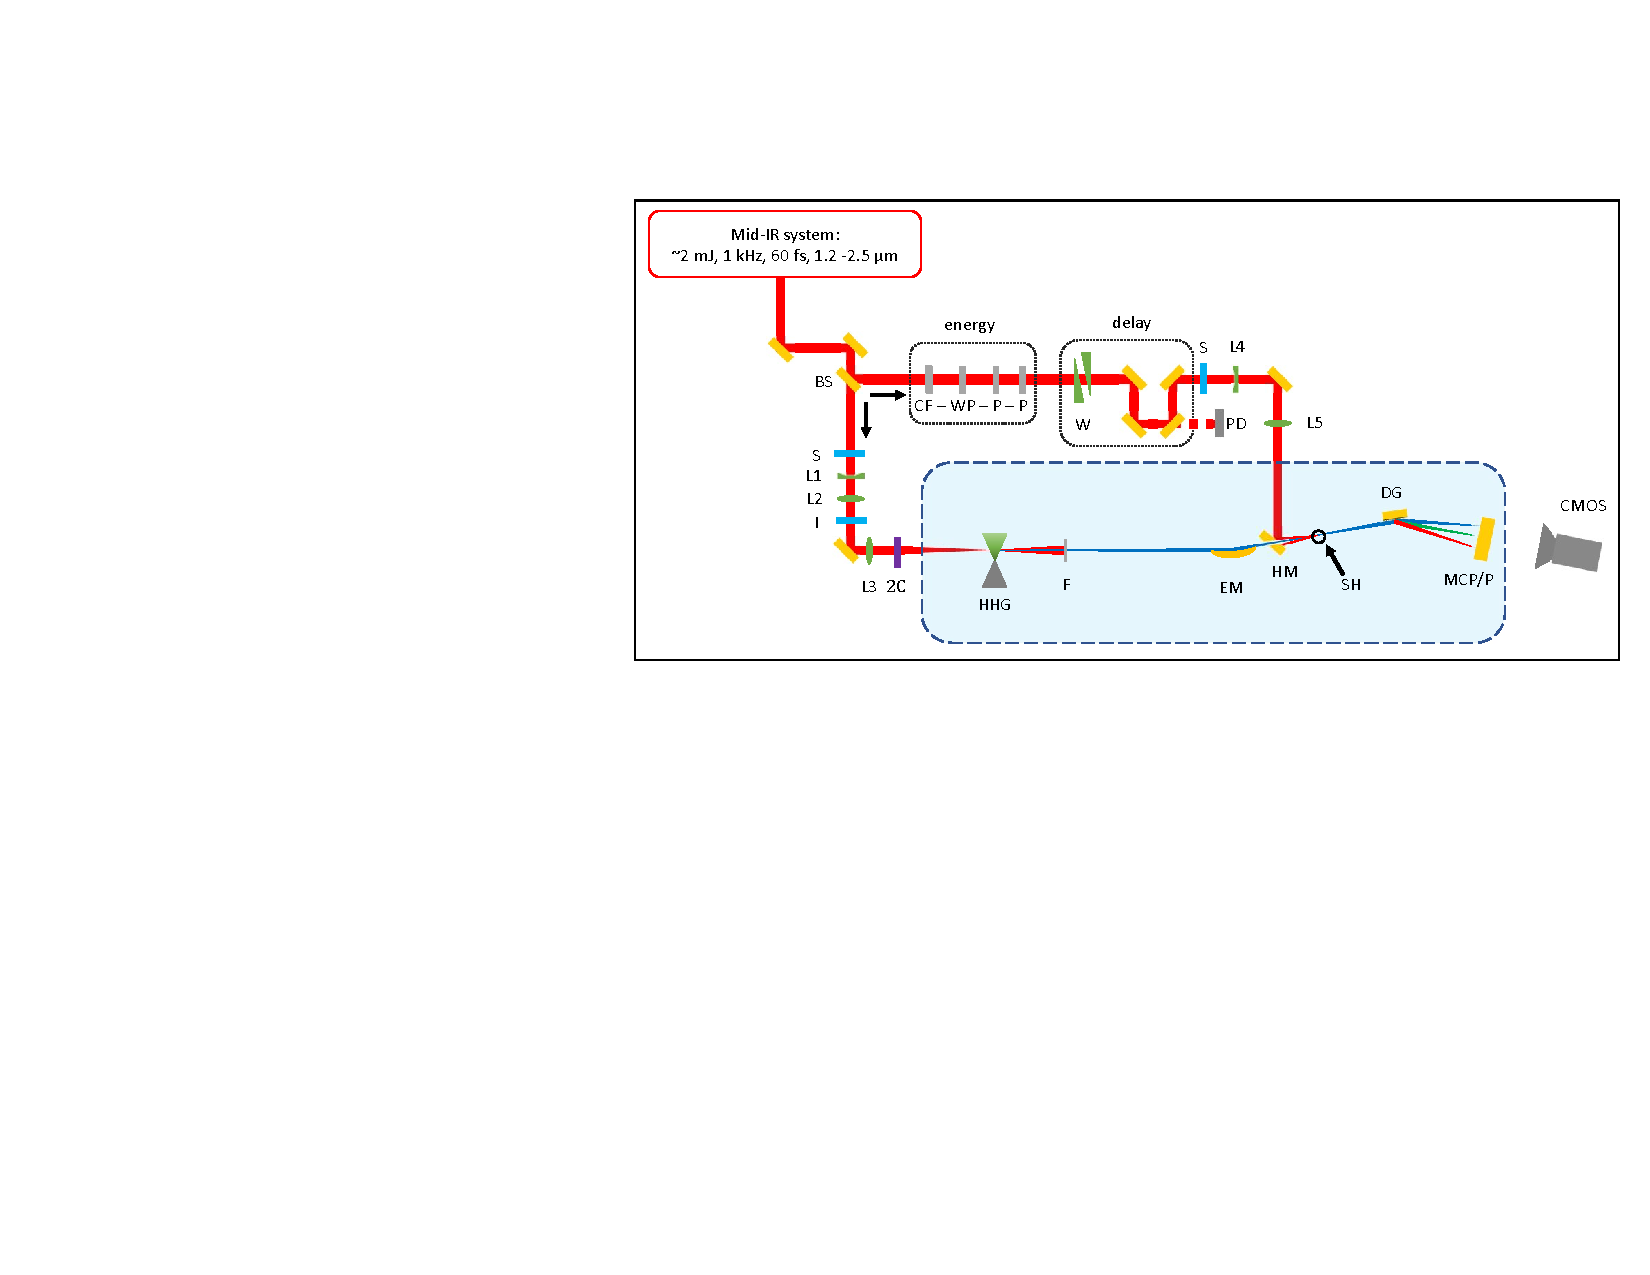
\includegraphics[width=0.95\textwidth]{figures/chap2/beamline_schematic.pdf}
	\caption{Schematic of the Transient Absorption BeamLine (TABLe). Blue shaded region represents vacuum. BS: beam splitter, S: computer-controlled shutter, L: lens, I: iris, 2C: optics for two-color generation, HHG: high harmonic generation, F: metallic filter, EM: ellipsoidal mirror, HM: hole mirror, SH: sample holder, CF: long-pass color filter, WP: $\lambda/2$ waveplate, P: wire-grid polarizer, W: delay wedges, PD: photodiode and associated optics, DG: dispersive grating, MCP/P: micro-channel plate and phosphor.}
	\label{fig:beamline_schematic}
\end{figure}

\subsection{Design Goals}
compare to the old attosecond beamline, cite razvan's thesis \cite{chirlaAttosecondPulseGeneration2011}. main differences between the new and old beamlines:

\begin{itemize}
	\item in-air pump design allows for complex optics (THz, OPA, etc.) in pump arm
	\item smaller vacuum chambers, easier to work inside
	\item not as well isolated from external environment (bellows feet not implemented)
	\item photon spectrometer, can accomodate simultaneous electron \& photon measurements
	\item modular endstation design
\end{itemize}


\subsection{XUV Optics}

\subsubsection{Fresnel Reflection from a Rough Surface}

\textbf{need a figure showing the interface, defining angles, indices, etc.}

We use the familiar Fresnel equations to model reflection from the surface of a conductive surface \cite{zangwillModernElectrodynamics2013}. In the equations that follow, the vacuum is denoted by $j=1$ and the conductive material is $j=2$. The incident electric field is $E_I$ and the reflected component is $E_R$. Following standard convention, the $p$-polarized light refers to light that has a polarization normal to the surface; $s$-polarized light is polarized parallel to the surface. The complex reflection amplitudes $r_{s,p}$ are written in terms of the complex impedance $\hat{Z}_j = \mu_j c / \hat{n}_j$ and the angle measured from the normal in each medium $\theta_j$:
\begin{equation}
\hat{r}_s \equiv \left[ \frac{E_R}{E_I} \right]_s = \frac{\hat{Z}_2 \cos \theta_1 - \hat{Z}_1 \cos \theta_2}{\hat{Z}_2 \cos \theta_1 + \hat{Z}_1 \cos \theta_2}
\label{eqn:Fresnel_rs_1}
\end{equation}
\begin{equation}
\hat{r}_p \equiv \left[ \frac{E_R}{E_I} \right]_p = \frac{\hat{Z}_1 \cos \theta_1 - \hat{Z}_2 \cos \theta_2}{\hat{Z}_1 \cos \theta_1 + \hat{Z}_2 \cos \theta_2}
\label{eqn:Fresnel_rp_1}
\end{equation}
Next, we assume non-magnetic media ($\mu_1=\mu_2=\mu_0$) and write the amplitudes in terms of the complex indices of refraction $\hat{n}_j = n_j + i k_j$:
\begin{equation}
\hat{r}_s = \frac{\hat{n}_1 \cos \theta_1 - \hat{n}_2 \cos \theta_2}{\hat{n}_1 \cos \theta_1 - \hat{n}_2 \cos \theta_2}
\label{eqn:Fresnel_rs_2}
\end{equation}
\begin{equation}
\hat{r}_p = \frac{\hat{n}_1 \cos \theta_2 - \hat{n}_2 \cos \theta_1}{\hat{n}_1 \cos \theta_2 + \hat{n}_2 \cos \theta_1}
\label{eqn:Fresnel_rp_2}
\end{equation}
The reflectance is the modulus squared of the reflection amplitudes:
\begin{equation}
\hat{R}_s = \left| \frac{\hat{n}_1 \cos \theta_i - \hat{n}_2 \cos \theta_t}{\hat{n}_1 \cos \theta_i - \hat{n}_2 \cos \theta_t} \right|^2
\label{eqn:Fresnel_Rs_1}
\end{equation}
\begin{equation}
\hat{R}_p = \left| \frac{\hat{n}_1 \cos \theta_t - \hat{n}_2 \cos \theta_i}{\hat{n}_1 \cos \theta_t + \hat{n}_2 \cos \theta_i} \right|^2
\label{eqn:Fresnel_Rp_1}
\end{equation}
Finally, we assume that the first medium is vacuum ($\hat{n}_1 = 1$) and apply Snell's law to write the transmitted angle $\theta_2$ in terms of the incident angle $\theta_1$:

\begin{equation}
\hat{R}_s = \left| \frac{\cos \theta_1 - \hat{n}_2 \sqrt{1-\left(\frac{1}{n_2}\sin \theta_1\right)^2}}{\cos \theta_1 + \hat{n}_2 \sqrt{1-\left(\frac{1}{n_2}\sin \theta_1\right)^2}} \right|^2
\label{eqn:Fresnel_Rs_2}
\end{equation}

\begin{equation}
\hat{R}_p = \left| \frac{\sqrt{1-\left(\frac{1}{n_2}\sin \theta_1\right)^2} - \hat{n}_2 \cos \theta_1}{\sqrt{1-\left(\frac{1}{n_2}\sin \theta_1\right)^2} + \hat{n}_2 \cos \theta_1} \right|^2
\label{eqn:Fresnel_Rp_2}
\end{equation}

The above analysis is valid for a perfectly smooth interface, but real optics have finite roughness. Loosely speaking, the surface roughness becomes important when it is on the order of the photon wavelength. As a point of comparison, a high quality off-the-shelf optic will have a surface roughness of $\lambda/10 = 63.2 \text{ nm}$, which is 5 times larger than the wavelength of a 100 eV photon. Clearly, we need specialized optics if we want to work in the XUV.

We will summarize the results of the analytic treatment of surface roughness in the literature \cite{sentenacStatisticalAspectsWave2009, gibaudSpecularReflectivitySmooth2009}. The surface roughness can be thought of as a local modulation $\delta z(\vec{r})$ of the ideal interface height $z(\vec{r})$ with a variance $\langle z^2 \rangle$, and a characteristic in-plane length scale $\delta r$ over which the modulation occurs. There are two limiting cases to consider, based on the relative magnitudes of $\delta r$ and the extinction length $1/k_2$. For reference, the extinction length is on the order of 1 $\mu m$ for hard x-rays, and about 10 nm for XUV light.

First, consider the case where the characteristic length scale of the roughness is much larger than the extinction length ($\delta r \gg 1/k_2$). In this case, the local electric field can be expressed in the following form:

\begin{equation}
E_j (x,y) = \left( A_j^+ \exp \left(i k_{j,z} z \right) +  A_j^- \exp \left( - i k_{j,z} z \right)  \right) \exp \left( i \omega t - \boldmath{k}_i in||.\boldmath{r_{||}} \right)
\label{eqn:DW_1}
\end{equation}

In \cref{eqn:DW_1}, $A_j^+ (A_j^-)$ denotes the amplitude of the incoming (outgoing) wave and $k_i in ||.r_{||} = k_j \cos \theta_j$ denotes ???.

Then, the incoming field does not 
\begin{equation}
r^{rough} = \frac{\langle A_1^+ \rangle_x}{A_1^-} = r \left\langle \exp \left( 2 i k_{1,z} z \right) \right\rangle = r \exp \left( -2 k_{1,z} \langle z^2 \rangle \right)
\label{eqn:DW_2}
\end{equation}

\cref{eqn:DW_2} is the Debye-Waller factor.

Then, the modulation is slow enough that there is a phase relationship between the incident and reflected fields over a large area. This is the Debye-Waller limit, and the reflectance is modified by a factor of $\exp \left( -4 k_1^2 \langle z^2 \rangle \right)$.

If the modulation length scale is much less than the extinction length ($\delta r \ll 1/k_2$) then there is no short-scale correlations between the electric field and the roughness. This is the Croce-N\'{e}vot limit, and the reflectance is modified by a factor of $\exp \left( -4 k_1 k_2 \langle z^2 \rangle \right)$.

For hard x-rays, the Nevot-Croce Surface roughness has the effect of reducing the reflectance by an exponential factor. 

The finite surface roughness of a real mirror reduces the reflectance by a factor of $\exp\left(-4 k_1^2 \sigma^2\right)$, called the \textit{Debye-Waller factor} \cite{gibaudSpecularReflectivitySmooth2009}. Here, $\sigma$ is the root-mean-square (rms) of the vertical roughness, and $k_1$ is the normal component of the wave-vector in vacuum. The final result is below:


Combining \cref{eqn:Fresnel_Rs_2,eqn:Fresnel_Rp_2} with \cref{eqn:DW_2} yields the reflectance of a rough metallic surface:

\begin{equation}
\hat{R}_s = \left| \frac{\cos \theta_1 - \hat{n}_2 \sqrt{1-\left(\frac{1}{n_2}\sin \theta_1\right)^2}}{\cos \theta_1 + \hat{n}_2 \sqrt{1-\left(\frac{1}{n_2}\sin \theta_1\right)^2}} \right|^2 \left( \frac{2 \pi \sigma \cos \theta_1}{\lambda} \right)^2
\label{eqn:Fresnel_Rs_3}
\end{equation}

\begin{equation}
\hat{R}_p = \left| \frac{\sqrt{1-\left(\frac{1}{n_2}\sin \theta_1\right)^2} - \hat{n}_2 \cos \theta_1}{\sqrt{1-\left(\frac{1}{n_2}\sin \theta_1\right)^2} + \hat{n}_2 \cos \theta_1} \right|^2 \left( \frac{2 \pi \sigma \cos \theta_1}{\lambda} \right)^2
\label{eqn:Fresnel_Rp_3}
\end{equation}



The mid spatial frequency roughness (MSFR) of the ellipsoidal mirror's surface is $\le0.3$ nm when sampled at a spatial frequency of 1-200 $\mu m$.

The extinction length in gold is on the order of 10 nm for photon energies below 500 eV. This length scale is much smaller than the spatial variation of the height of our ellipsoidal mirror (1 - 200 $\mu m$), so we treat the using the Debye-Waller factor \cite{stoevReviewGrazingIncidence1999,gibaudSpecularReflectivitySmooth2009}:

\begin{equation}
r^{rough} = r^{smooth} \exp \left( -2 k_{z,0} k_{z,1} \sigma^2 \right)
\end{equation}


- the extinction length for photon range 30 - 500 eV in gold is on the order of 0.07 - 0.2 nm.
- the 0.3 nm rms roughness is based on a measurement frequency of 1 - 200 microns. this corresponds to a relatively long-range / slowly varying roughness.
- therefore we should use the debye-waller factor.



Nevot-Croce model assumes random vertical roughness with a Gaussian distribution. for the low spatial frequencies of the roughness spectrum, the Fresnel reflection coefficient is usually multiplied with a Debye-Waller factor $\exp\left(-16 \pi^2 k_1^2 \sigma^2\right)$, while for the high spatial frequencies, the correction coefficient is given by the Nevot-Croce correction factor $\exp\left(-16 \pi^2 k_1 k_2 \sigma^2\right)$, where $\sigma$ is the root-mean-square (rms) of the vertical roughness, and $k_1$ and $k_2$ are the normal components of the wave-vectors in the two media \cite{stoevReviewGrazingIncidence1999}.



FRED calculations: toroid demagnification vs ellipsoid demagnification

why an ellipsoid doesn't have aberrations

aligning the ellipsoidal mirror - what the spot looks like when misaligned

\subsubsection{Material Choice}
\begin{figure}
	\centering
	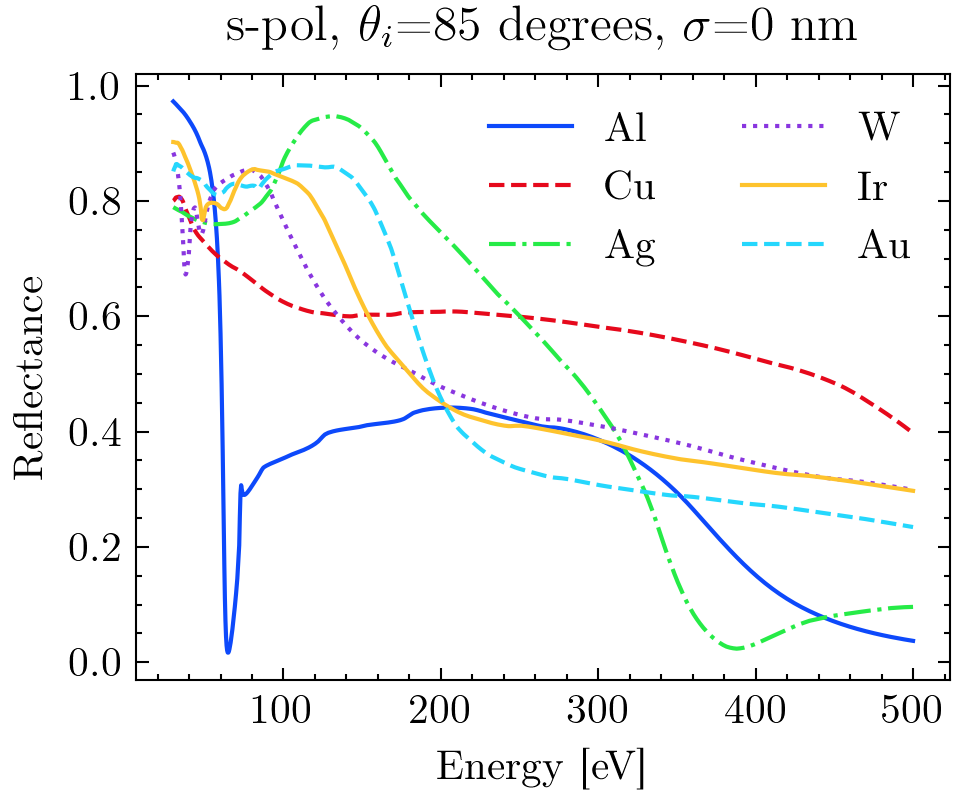
\includegraphics[width=0.75\textwidth]{figures/chap2/Fresnel_NoSigma.png}
	\caption{Fresnel reflectance for s-polarized light on smooth metal mirrors at a grazing angle of 5 degrees. Refractive index data obtained from \cite{gulliksonCXROXRayInteractions,henkeXRayInteractionsPhotoabsorption1993}. Calculation follows \cref{eqn:Fresnel_Rs_2,eqn:Fresnel_Rp_2}.}
	\label{fig:Mirror_Material_Choice}
	% generated using Fresnel.py
\end{figure}

\cref{fig:Mirror_Material_Choice} shows the Fresnel reflectance from various materials with an ideal interface at fixed angle. While other materials provide have better reflectance, gold was chosen due to its chemical inertness. 

We compare two common materials.

Gold was chosen due to its chemical inertness and generally good reflectivity.

thickness of gold layer -- penetration depth (in general and at 5 degrees)

40 nm of gold with a sticking layer ... explain your reasoning

\subsubsection{Angle Choice}
\begin{figure}
	\centering
	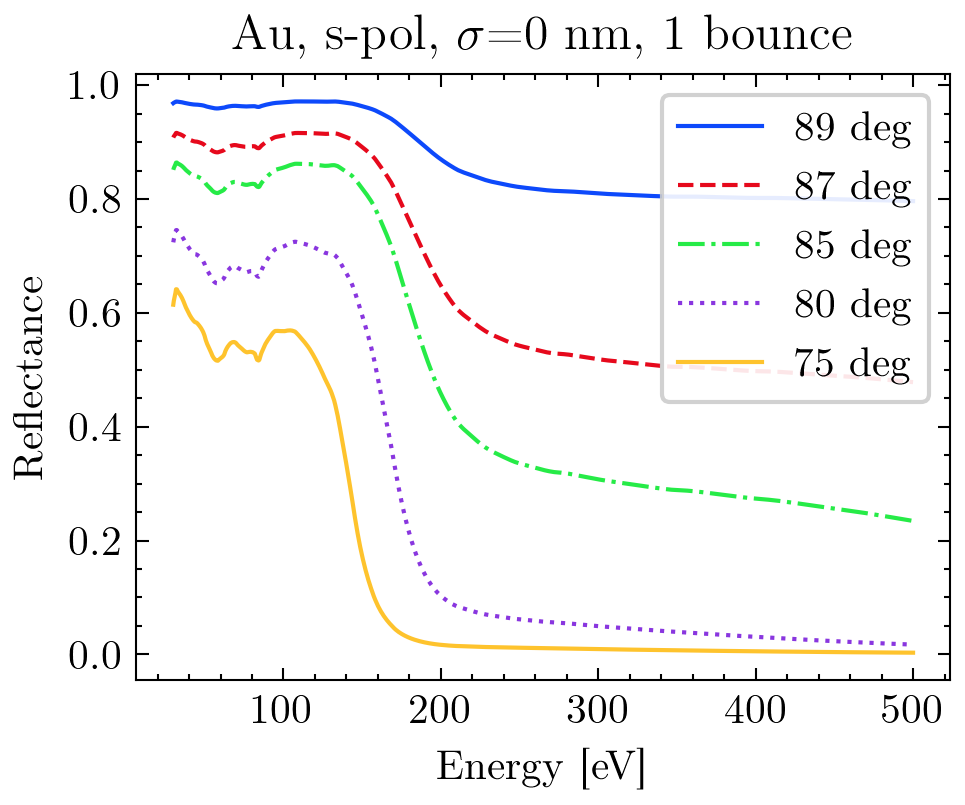
\includegraphics[width=0.75\textwidth]{figures/chap2/Au_ReflvsAngle.png}
	\caption{Fresnel reflectance for $s$-polarized light from a single smooth gold mirror as a function of incident angle. Calculation follows \cref{eqn:Fresnel_Rs_2,eqn:Fresnel_Rp_2}.}
	\label{fig:Au_ReflvsAngle}
	% generated using Fresnel.py
\end{figure}

\begin{figure}
	\centering
	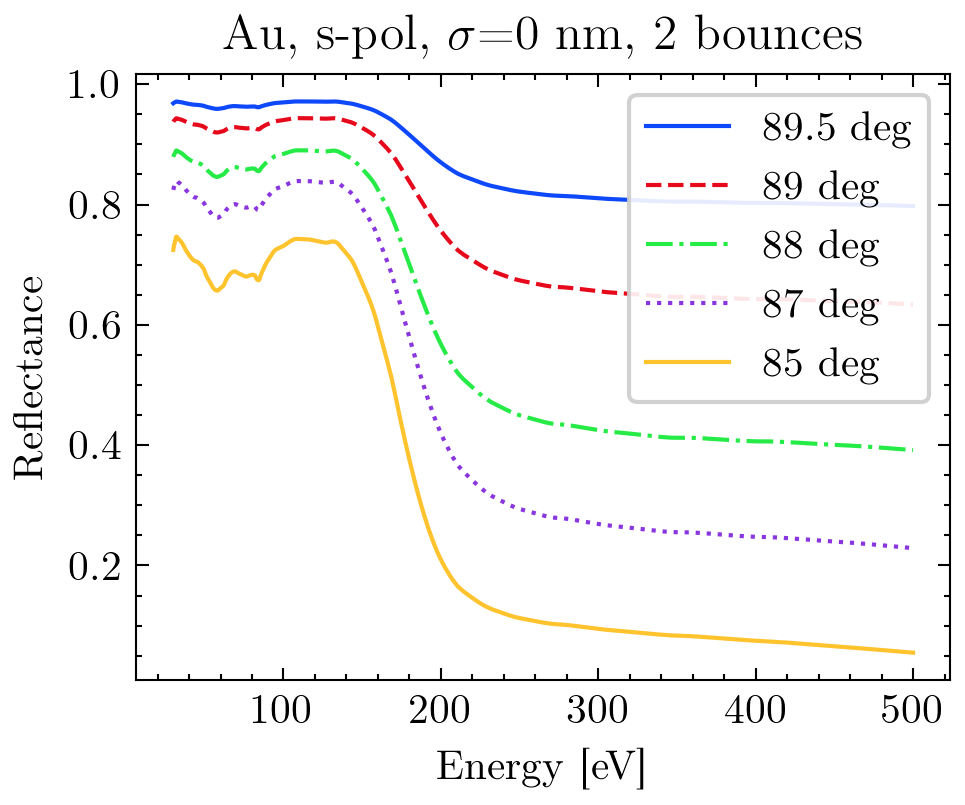
\includegraphics[width=0.75\textwidth]{figures/chap2/Au_ReflvsAngle_2bounce.png}
	\caption{Fresnel reflectance for $s$-polarized light from two smooth gold mirrors as a function of incident angle. Calculation follows \cref{eqn:Fresnel_Rs_2,eqn:Fresnel_Rp_2}.}
	\label{fig:Au_ReflvsAngle_2bounce}
	% generated using Fresnel.py
\end{figure}

why did we go with 5 degrees?

footprint of beam on the optic / size of the optic \cite{gibaudSpecularReflectivitySmooth2009}:
\begin{equation}
F = \frac{t_1}{\sin \alpha}t_2
\label{eqn:EM_footprint}
\end{equation}
in the above equation, $t_1, t_2$ are the rectangular dimensions of the input beam and $\alpha$ is the grazing angle of the light. then $F$ is the footprint of the beam on the angled mirror.

5 degrees was a good compromise between reflectivity, footprint on optic, and footprint of optic

\subsubsection{Roughness Choice}
\begin{figure}
	\centering
	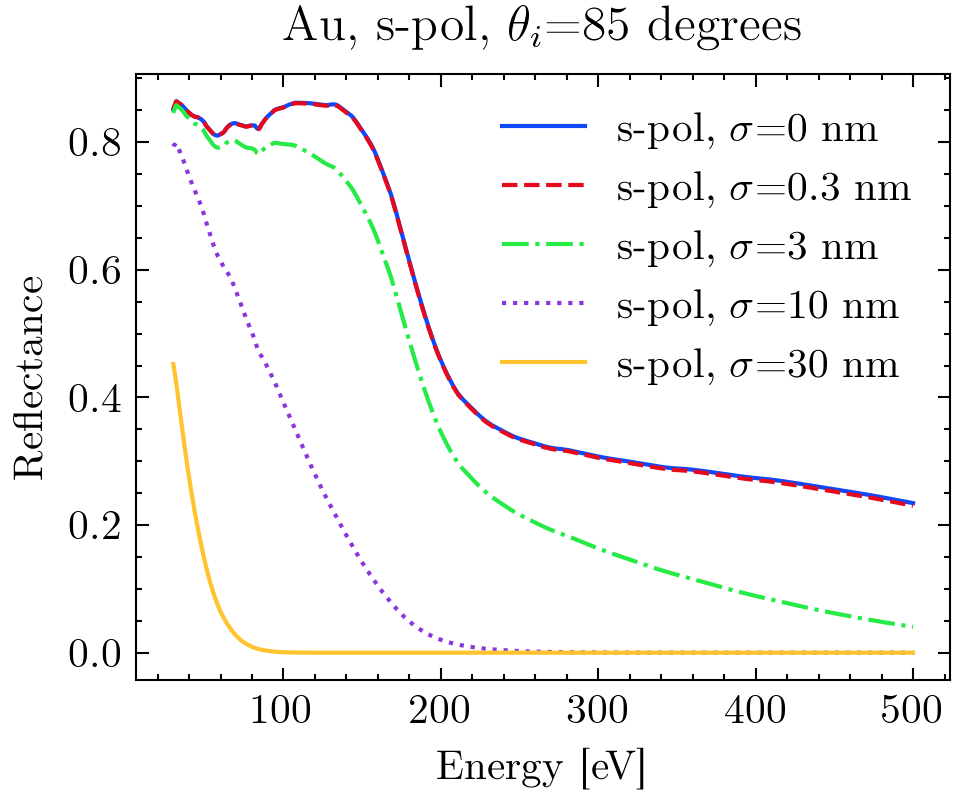
\includegraphics[width=0.75\textwidth]{figures/chap2/R_vs_roughness.png}
	\caption{Effect of surface roughness on reflectance. Calculation follows \cref{eqn:Fresnel_Rs_3}.}
	\label{fig:R_vs_roughness.png}
	% generated using Fresnel.py
\end{figure}

why did we go with 0.3 nm rms? because it was state of the art, and very close to the performance of a ideal/smooth surface

\subsection{Types of Reflective Optics}

\subsubsection{compare toroid, ellipsoid and multilayer mirrors}

\subsubsection{our ellipsoidal mirror specifications}

\subsubsection{FRED simulations of the ellipsoidal mirror focus}

\subsection{IR Optics for the Generation Chamber}

optics: CaF2 window. focusing geometry: supported focal lengths, telescope, 2-color generation. XYZ translation stage and modular gas nozzle holder.

\subsection{IR Optics for the Pump Arm}

\subsubsection{hole mirror}
the need for collinear IR-XUV geometry (spatial overlap, temporal smearing)

HM placement: before or after EM?

\subsubsection{description of optics used}

\subsubsection{Calculation of IR intensity at Focus}

\begin{figure}
	\centering
	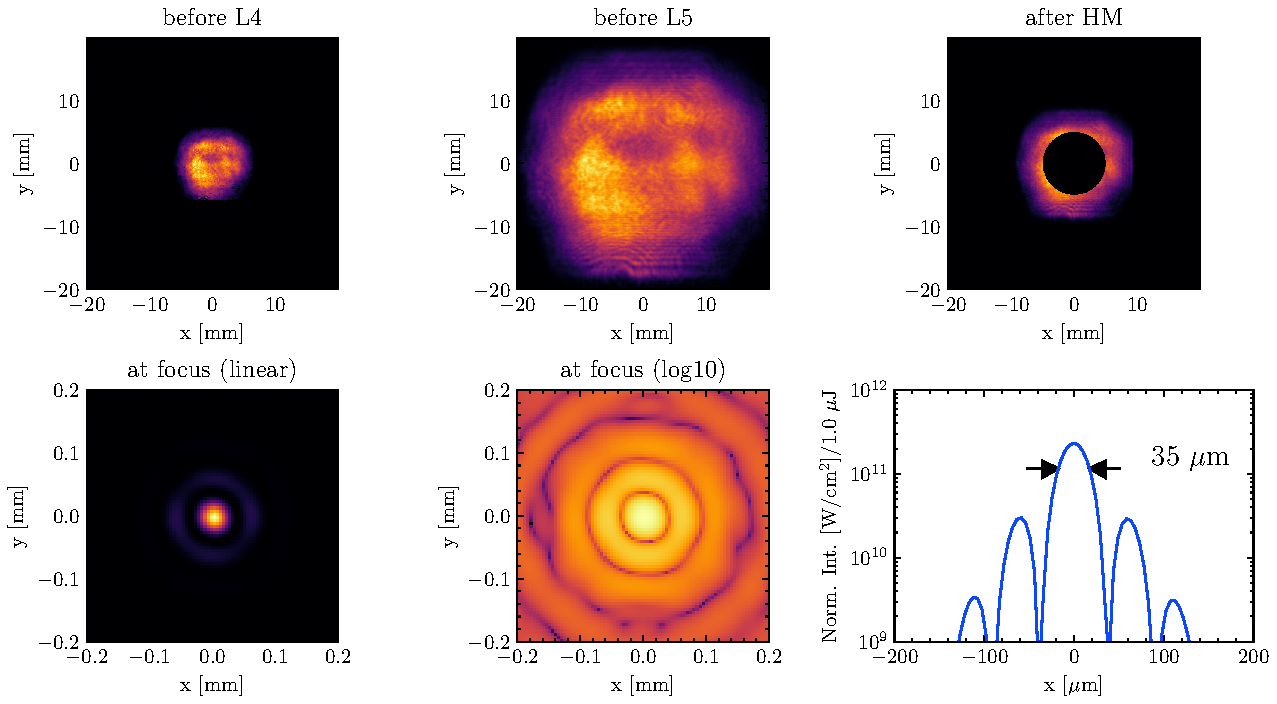
\includegraphics[width=0.75\textwidth]{figures/chap2/pump_on_focus_calculation_8192_inferno.pdf}
	\caption{Numerical propagation of the IR ($\lambda$=1500 nm) beam through the pump arm. Beam path layout follows \cref{fig:beamline_schematic}. Each panel shows the intensity of the beam as the beam propagates towards the focus. The first panel shows the measured intensity (Electrophysics PV320 thermal camera), all other panels are calculations. The arrows on the lineout indicate the FWHM. All calculations are for vacuum ($n=1$). See text for details.}
	\label{fig:pump_on_focus_calculation}
	% plot made with \Python Scripts\LightPipes\pump_intensity.py using N=2**13 gridside
\end{figure}

The profile of the TOPAS output at $\lambda$=1500 nm was measured immediately before the pump arm's diverging lens (L4 in \cref{fig:beamline_schematic}) using an Electrophysics PV320 thermal camera. The beam was propagated numerically using the Python package \textit{Lightpipes for Python} \cite{vdovinLightPipesPython} through the remainder of the pump arm to the focus using a grid size of $2^{13}\times2^{13}$. The result of this calculation is shown in \cref{fig:pump_on_focus_calculation}. Optical element parameters are as follows: L5 is a $f = +500 \text{ mm}$ Thorlabs LA1380-C, located 68.5 cm after L4 ($f = -300 \text{ mm}$, Thorlabs LF1015-C). The hole mirror HM is located 53 cm after L5 and has an inner radius of 5 mm. Clear apertures of 22.86 mm (L4), 45.72 mm (L5) and 50.8 mm (HM) were used. A 65 fs Gaussian temporal profile containing 1 $\mu$J of energy was assumed.

Reflection losses from 2 Ag mirrors, 2 AR-coated lenses and uncoated $\text{CaF}_2$ vacuum window are responsible for a 26.2\% reduction in transmitted power. Additionally, the geometry of the hole mirror causes only 56\% of incident power to be incident on a reflective surface (the rest is lost to the central aperture). In total, the pump arm transmits 41.3\% of the power from before L4 to the focus.

The IR intensity makes an Airy-like diffraction pattern at the focal plane. There is an intense bright spot surrounded by a series of rings, with the intensity of each ring as the distance from the center increases. The rings exhibit a periodic modulation in intensity with respect to angle $\phi$. This four-fold symmetry is due to the square-like spatial profile of the TOPAS output, whereas the clipping from the hole mirror's aperture is responsible for the central peak and ring structure. The central lobe has a peak intensity of $\sim 2.3 \times 10^{11} \text{ W/cm}^2$ per 1 $\mu$J input pulse energy and a FWHM of 35 $\mu$m. The first ring has a radius of 59 $\mu$m and a peak intensity $\sim 2.9 \times 10^{10} \text{ W/cm}^2$ per input $\mu$J pulse energy. Thus the central lobe's peak intensity is about an order of magnitude larger than the ring's intensity. However, the central spot only contains about 49\% of the total power, as the rings cover a much larger area.

Note that the above calculations assume perfect alignment into the hole mirror (i.e., the IR beam is centered on the central aperture of the hole mirror). If the IR beam is misaligned to the hole mirror, then the transmission to the focus will increase as the most intense part of the beam is no longer clipped by the central aperture. Therefore, a drift in the laser's pointing during an experiment can effect the sample's interaction intensity.


\subsection{Pulse energy control, calibration \& monitoring}

\subsection{Delay control \& calibration}

\subsection{XUV-IR spatial overlap}

\begin{figure}
	\centering
	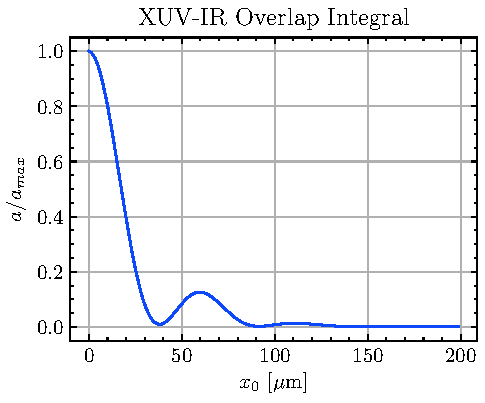
\includegraphics[width=0.5\textwidth]{figures/chap2/XUV-IR_overlap_integral.pdf}
	\caption{XUV-IR overlap function, as defined in \cref{eqn:XUV-IR_integral}, calculated using the numerical simulation results of \cref{fig:pump_on_focus_calculation} and a Gaussian XUV beam with a 6 $\mu$m waist. The result has been normalized to perfect overlap, $a_{max}$.}
	\label{fig:XUV-IR_integral}
	% plot made with \Python Scripts\LightPipes\pump_intensity.py using N=2**13 gridside
\end{figure}

\textbf{need to re-write this intro paragraph. excitation fraction hasn't been computed yet}

The excitation fraction can be computed for each spatial coordinate on the sample using the above method and the predicted intensity distribution from the numerical beam propagation calculations. Because the electrons are being excited via a single-photon process, the excited carrier density will be proportional to the fluence, and thus proportional to the intensity shown in \cref{fig:pump_on_focus_calculation}. Because the intensity of the XUV is very weak, the absorption of the XUV by the sample is also linear. Thus, we should expect the ATAS signal to be proportional to the XUV-IR overlap integral:
\begin{equation}
a = \frac{ \int dV \text{ } I_{\text{IR}} I_{\text{XUV}} }{ \int dV \text{ } I_{\text{IR}} \int dV \text{ } I_{\text{XUV}} }
\label{eqn:XUV-IR_integral_volume}
\end{equation}
Here, the integration volume is over the entire sample. If we assume that the intensity distribution does not appreciably change over the thickness of the sample, we can simplify the above equation. This is a reasonable assumption because the sample ($L = 100 \text{ nm}$) is much thinner the Rayleigh range ($z_R \sim 1 \text{ mm}$), and the absorption is low ($\sim 4\%$). So we assume the sample is a $\delta$-function in thickness and only evaluate the intensities at the focal plane. With this assumption, the overlap integral becomes:
\begin{equation}
a = L \frac{ \int dA \text{ } I_{\text{IR}} I_{\text{XUV}} }{ \int dA \text{ } I_{\text{IR}} \int dA \text{ } I_{\text{XUV}} }
\label{eqn:XUV-IR_integral}
\end{equation}
Knife edge measurements have been performed on the XUV light, showing that it has a Gaussian spatial profile with a beam waist of 6 $\mu$m. We write down the spatial profile of the XUV light at the focus:
\begin{equation}
I^{XUV} = I_0^{XUV} \exp \left( - 2 ((x-x_0)^2 + (y-y_0)^2) /  w_{XUV}^2 \right)
\end{equation}
Here, $I_0^{XUV}$ is the peak intensity and $w_{XUV}$ is the beam waist (radius), defined as the point where the intensity falls to $e^{-2} = 13.5\%$ of its maximum. The lateral shift from the center of the IR focal spot in the horizontal and vertical directions is $x_0$ and $y_0$, respectively. With this formulation, and using the simulation results for the IR spot, the XUV-IR overlap integral is calculated as a function of XUV-IR misalignment $(x_0, y_0)$. This result is shown in \cref{fig:XUV-IR_integral}. Here, XUV beam is translated relative to the IR beam in the horizontal direction ($x_0$ with $y_0=0$) and the overlap is computed from \cref{eqn:XUV-IR_integral}.

\cref{fig:XUV-IR_integral} shows the sensitivity of a condensed matter ATAS experiment to relative alignment.\footnote{Note that the relevant parameter in \cref{eqn:XUV-IR_integral} is the relative positions of the two focal spots. We have yet to calculate the sensitivity of spatial overlap to deviations in the input laser pointing.} A spatial overlap deviation of 10 $\mu$m will cause the XUV-IR overlap - and thus the measured signal - to drop by 20\%. Note that a 10 $\mu$m displacement of the IR at the sample corresponds to a 15 $\mu$rad tilting of the hole mirror (HM). There are two ways misalignment can affect experimental results. If the relative positions of the XUV and IR focal spots changes as an experiment is performed, then the recorded ATAS signal would be a function of both the laser-induced dynamics and the XUV-IR spatial misalignment. On the other hand, if the entire experiment is performed using a constant misalignment, we would be exciting the sample to some peak excitation fraction $f$, but our probe would be measuring a lower excitation fraction ($\approx f a / a_{max}$). Consequently, the measured ATAS signal would be lower than otherwise expected, and any attempts to boost the signal by increasing the interaction intensity could result in permanent laser-induced sample damage.

A condensed matter ATAS experiment has much tighter alignment tolerances than a gas phase experiment. This discrepancy is a simple consequence of sample geometry and density. In either experiment, the measured signal comes from the region of space where the sample density, XUV intensity and IR intensity overlap. The transmission of XUV through the sample is, to first order, $T= \exp(- n \mu_a d)$, where $n$ is the number density, $d$ is the sample thickness and $\mu_a$ is the photoabsorption cross section. As discussed above, for technical reasons the experiment should be designed with $T \approx 1/2$. Therefore, the product $n \mu_a d$ will be approximately constant for any transient absorption experiment.

The number density of a condensed phase sample is determined by the chemistry of the compound and is on the order of $4 \times 10^{22} \text{ atoms}/\text{cm}^3$. The experimentalist is free to engineer clever sample geometries, heterostructures and/or nanopatterns, but the high atomic density (and thus absorption coefficient) dictates a total sample thickness on the order of 100 nm. On the other hand, the spatial profile and density of a gas phase sample is determined by the gas nozzle design and its backing pressure, respectively. A typical nozzle used in our lab produces a gas plume with lateral dimensions on the order of 200 - 500 $\mu$m. This effectively creates a sample that is three orders of magnitude thicker than a condensed phase sample, which relaxes the alignment constraints significantly. This has important consequences for the alignment of the sample.

If the XUV and IR are perfectly collinear, then the beam overlap region is effectively infinite in the propagation direction. In this case, the XUV-IR overlap integral will be positive regardless of any displacement of the sample plane from the focal plane, and maximal when the sample lies in the focal plane. However, if there is a small angle $\delta \theta$ between their $k$-vectors, then the beams will only spatially overlap within a finite region. In this case, the position of the sample plane relative to the beam crossing plane becomes a critical experimental parameter. For an infinitely thick sample (i.e., a chamber effusively filled with gas), it wouldn't matter where the beams crossed as long as they overlapped somewhere within the chamber. Then, the overlap integral would decrease as a function of $\delta \theta$, but it would never go to zero. For a thin sample, the bounds of \cref{eqn:XUV-IR_integral_volume} must enclose the beam overlap region, or else the integral will be zero. Thus, the signal strength of a condensed phase ATAS experiment is roughly 3 orders of magnitude more sensitive to the $z$-position of the sample relative to the focal plane than a gas phase ATAS experiment.


\section{XUV Photon Spectrometer}
\label{sec:XUV_spectrometer}


\subsection{basic description}

\subsection{2D CMOS sensor}

\subsection{Spectral Calibration}

\section{old stuff}


All elements in the periodic table have at least one electronic transition between 30 and 500 eV. Each transition has a characteristic photoabsorption cross section line shape, resulting in poor (good) transmission above (below) the transition. In the terminology of x-ray spectroscopy, this spectroscopic feature is called an \textit{x-ray absorption edge}. Typical attenuation lengths\footnote{The attenuation length is defined as the depth into the material measured along the surface normal where the intensity of x-rays falls to $1/e$ of its value at the surface.} for most elements near an edge at energies of interest to our lab are measured in the tens of nanometers.

This basic feature of XUV light-matter interaction is both a blessing and a curse. On one hand, we can exploit the strong absorption to perform element-specific transient absorption spectroscopy on a myriad of elements and compounds (materials science permitting). On the other hand, the strong absorption puts severe experimental limits on any apparatus that uses XUV.




modular endstation design

in-air convenience

- split level table

- magnetic turbo pumps


\section{XUV Optics}

The XUV light is divergent after its generation and needs to be focused onto a sample for the experiment. The short relatively wavelength of the XUV puts strong requirements on the surface quality of the focusing optic, raising the cost and manufacturing time significantly. Alignment of the optic is frustrated by the need for in-vacuum propagation and the invisible nature of XUV light. These factors lead us to pursue a "one size fits all" broadband optic rather than a series of interchangeable narrow bandwidth optics tailored for individual experiments.

The presence of strong absorption edges over the bandwidth of the XUV pulse precludes the use of transmissive optics. Narrow bandwidth transmissive optics have been designed to exploit the dispersion near an absorption edge \cite{drescherExtremeultravioletRefractiveOptics2018}. However, these techniques cannot be extended to support the entire bandwidth of our XUV pulses. Reflective dielectric coatings have been designed for the XUV (\textbf{citation needed - Dietrich, Krauss?}), but their reflectance is only good for 10-20 eV (\textbf{need a source. this range might be incorrect.}). These considerations leave reflective optics as the only good choice for broadband XUV light.

The IR intensity profile at the focus is an important parameter for every experiment. In a transient absorption experiment, the experimental signal originates from the spatial overlap of the sample, the XUV and the IR light in the interaction region. Ideally, neither pulse would have any spatial structure at the interaction plane. In the real world, we design the optics to minimize the intensity variation of the IR over the spatial extent of the XUV spot. For finite beam sizes, this is accomplished by focusing the XUV tighter than the IR while minimizing aberrations. We chose to demagnify the XUV spot size by a factor of three, which reduces the XUV spot area by a factor of nine. This allows us to more strongly focus the IR pump pulse, resulting in a nine-fold increase of interaction intensity without changing the relative spot sizes of the XUV and the IR. While not required for a condensed matter experiment, the increased IR intensity was essential to doubly ionize helium gas for $e-2e$ experiments \cite{kiesewetterDynamicsNearThresholdAttosecond2019}.

In the following sections, we outline the decision-making process for choosing an XUV optic. We start with a review of the physics of reflection from a rough metallic surface. Using these results we determine the optimal material, thickness, surface roughness and angle of the optic. We then compare the most common mirror configurations and discuss their suitability for a 3x demagnification. We conclude by describing 



\subsection{XUV mirror choices}
%\begin{figure}
%	\centering
%	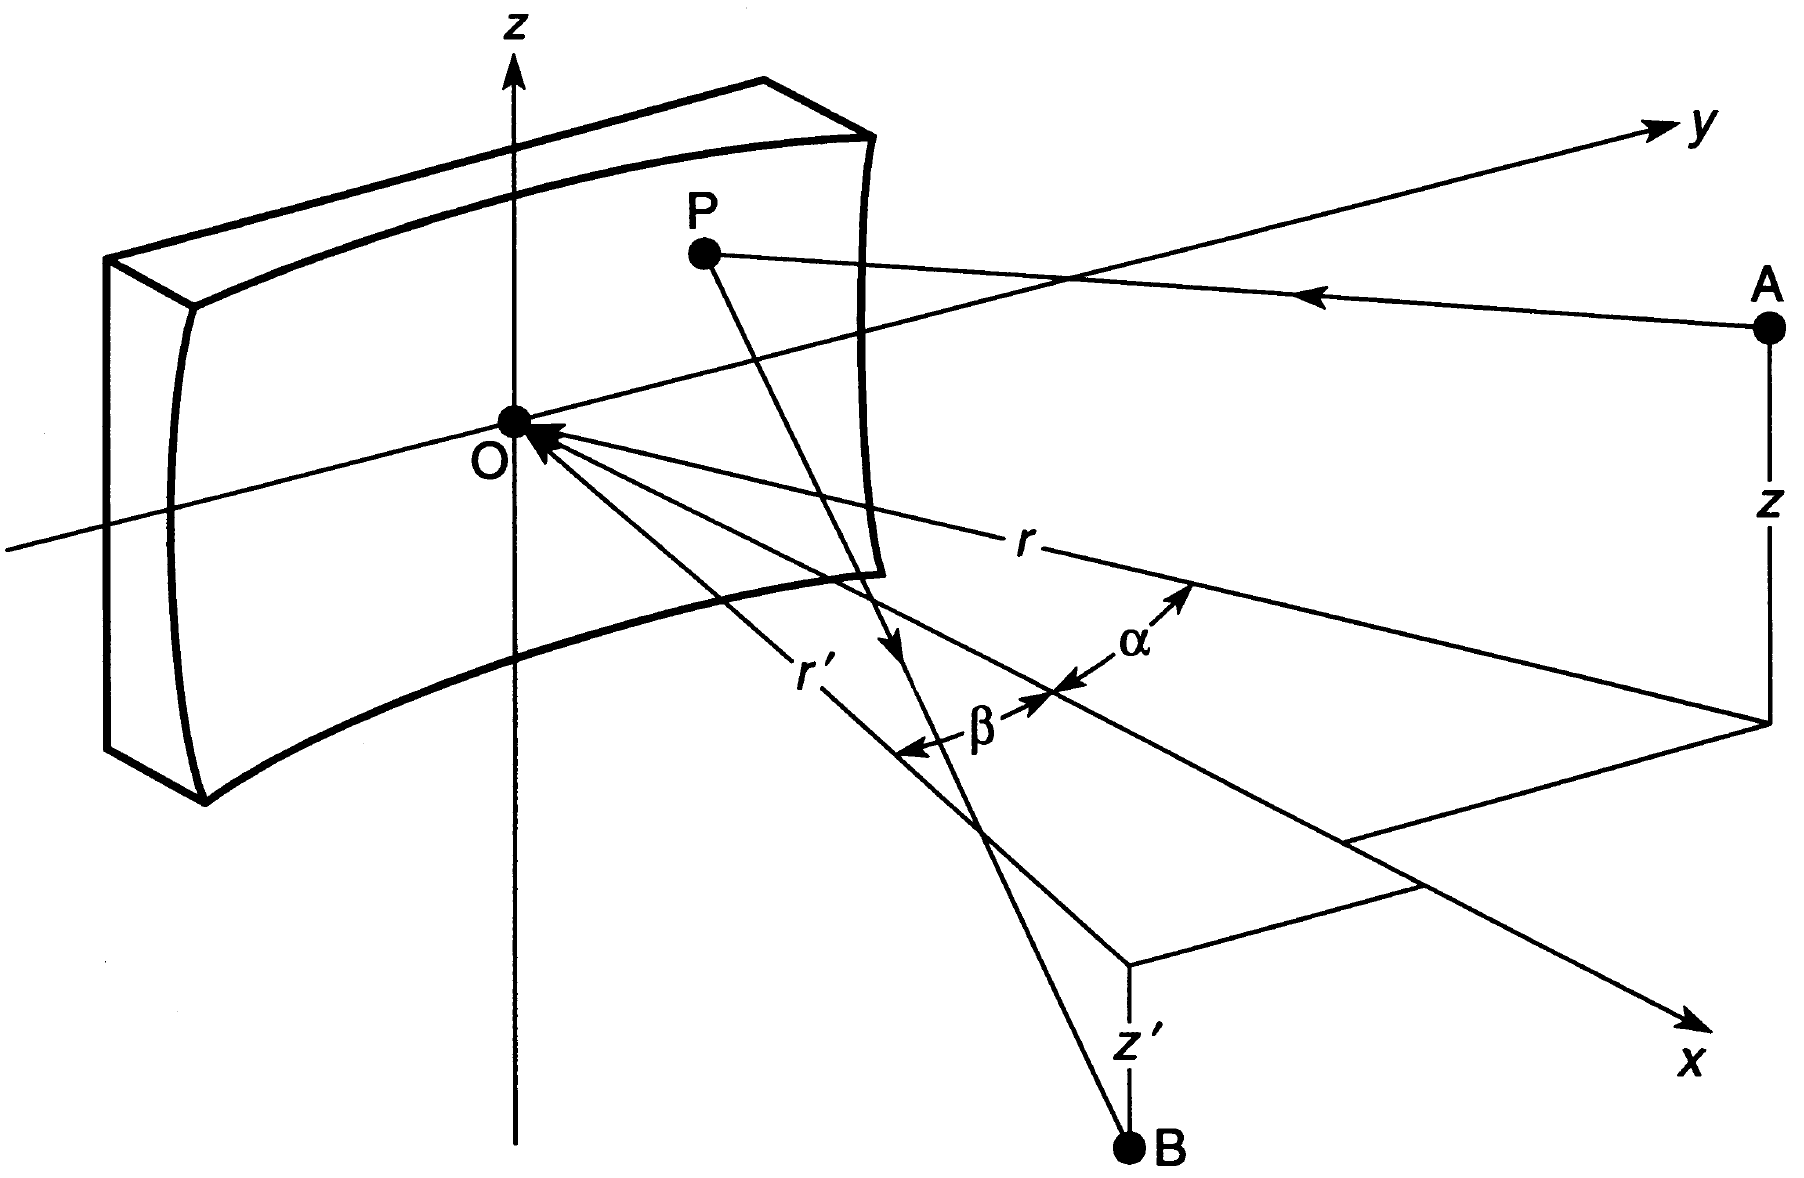
\includegraphics[width=0.75\textwidth]{figures/chap2/howells_FigA1.png}
%	\caption{Rectangular coordinate system used to discuss the optical light path function analysis. The center of the optic coincides with the origin $O$. Light from source point $A(x,y,z)$ strikes the mirror's surface at point $P(w,l, \xi)$ and leaves the system at point $B(x', y',z')$. Figure adapted from \cite{howellsMirrorsSynchrotronRadiationBeamlines1994}.}
%	\label{fig:LPF_coordinates}
%	% snipped from \cite{howellsMirrorsSynchrotronRadiationBeamlines1994}.
%\end{figure}

As discussed above, we are restricted to smooth grazing incident angle metallic mirrors, but the shape this mirror has not yet been discussed. We considered several focusing geometries for our beamline before ultimately choosing an ellipsoidal mirror. Spherical mirrors introduce significant aberration when operated away from normal incidence. Toroidal mirrors, when operated in a $2f-2f$ configuration, can re-image the source point without introducing any aberrations at the focus \cite{chirlaAttosecondPulseGeneration2011}. Additionally, the toroid's constant curvature allows it to be manufactured to a higher degree of accuracy than other shapes \cite{howellsMirrorsSynchrotronRadiationBeamlines1994}. However, toroids introduce significant coma when the entrance and exit arms are unequal (i.e., when $M\ne1$). These aberrations can be minimized by using a two-toroid configuration, but this introduces other problems. The second bounce greatly reduces the transmission of the optical system as a whole, as shown in \cref{fig:Au_ReflvsAngle_2bounce}. The reflection losses of the second optic could be offset by reducing the grazing angle of the pair, but at the cost of increasing the footprint of each optic. For example, an optic pair must operate at 88 degrees to achieve the reflectivity of a single optic at 85 degrees. Applying \cref{eqn:EM_footprint}, we can see that for a fixed input beam size, this 3 degree change increases the required dimensions of each mirror by 250\%. Even if the spacing between the two mirrors was negligible, a two-optic solution would increase the overall footprint of the refocusing system by a factor of 5. Furthermore, the presence of an additional reflective optic within the interferometer reduces the interferometric stability and makes the optical alignment of the system more difficult. The above arguments can also be applied to Kirkpatrick-Baez (KB) pairs \cite{kirkpatrickFormationOpticalImages1948} or other two-optic configurations. clearly a single optic solution was required.

%\subsubsection{unnecessary detail: delete}
%
%Fermat's principle can be applied to reflective optics to quantify geometric aberrations at the focus \cite{nodaGeometricTheoryGrating1974a,howellsMirrorsSynchrotronRadiationBeamlines1994}. To this end, the mirror surface can be analytically expressed as a Maclaurin series using the coordinate system in \cref{fig:LPF_coordinates}:
%\begin{equation}
%x = \sum_{i,j = 0} a_{ij} y^{i} z^{j}
%\end{equation}
%Here, all of the information about the surface of the optic is contained within the coefficients $a_{ij}$. Let $F$ be the optical path length for light originating at source point $A$, reflecting from mirror surface point $P$ and ending at exit point $B$. That is, let $F = AP + PB$. We can express $F$ as a series expansion in terms of the surface coordinates $w$ and $l$:
%\begin{dmath}
%F = w F_{100} + w F_{102} + l F_{011} + \frac{1}{2} w^2 F_{200} + \frac{1}{2} l^2 F_{020} + \frac{1}{2} w^3 F_{300} + \frac{1}{2} w l^2 F_{120} + w l F_{111} + \frac{1}{8} w^4 F_{400} + \frac{1}{4} w^2 l^2 F_{220} l^2 + \frac{1}{8} l^4 F_{040} + \frac{1}{4} w^2 F_{202} + \frac{1}{4} l^2 F_{022} + \frac{1}{2} l^3 F_{031} + \frac{1}{2} w^2 l F_{211} + \cdots
%\label{eqn:light_path_function}
%\end{dmath}
%According to Fermat's principle,
%\begin{equation}
%\pdv{F}{w} = \pdv{F}{l} = 0
%\end{equation}
%
%We consider the situation of a point source in the symmetry plane of the mirror ($z=z'=0$ and $k=0$), which is applicable for our beamline. Then, blurring at the focus occurs when $\Delta y_{ij0}^{'} \ne 0$ or $\Delta z_{ij0}^{'} \ne 0$:
%\begin{equation}
%\Delta y_{ij0}^{'} = \frac{r'}{\cos \alpha} \left( \pdv{F}{w} \right)_{ij0}
%\end{equation}
%\begin{equation}
%\Delta z_{ij0}^{'} = r' \left( \pdv{F}{l} \right)_{ij0}
%\end{equation}


connection between aberrations and temporal smearing \cite{bourassin-bouchetHowFocusAttosecond2013}

\subsubsection{KB pairs}
\begin{figure}
	\centering
	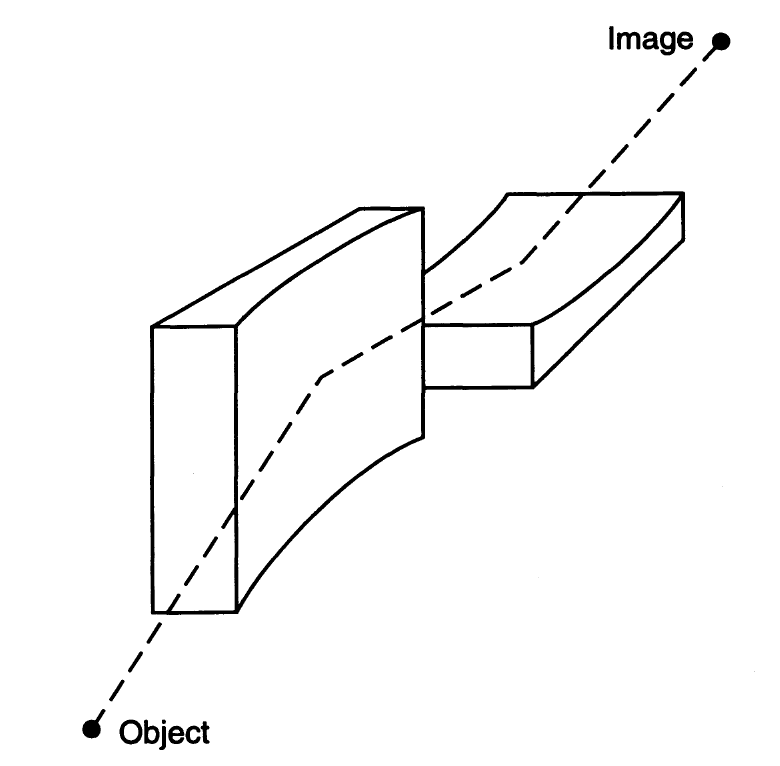
\includegraphics[width=0.75\textwidth]{figures/chap2/KB_geometry_Howells1994.png}
	\caption{placeholder text.}
	\label{fig:KB_geometry_Howells1994}
	% snipped from Howells 1994
\end{figure}

original citation \cite{kirkpatrickFormationOpticalImages1948}

geometric description

avoided due to size of optics

disadvantage: multi-mirror configuration. difficult to align, extra bounce causes more reflection losses.

\subsubsection{toroidal mirrors}
\begin{figure}
	\centering
	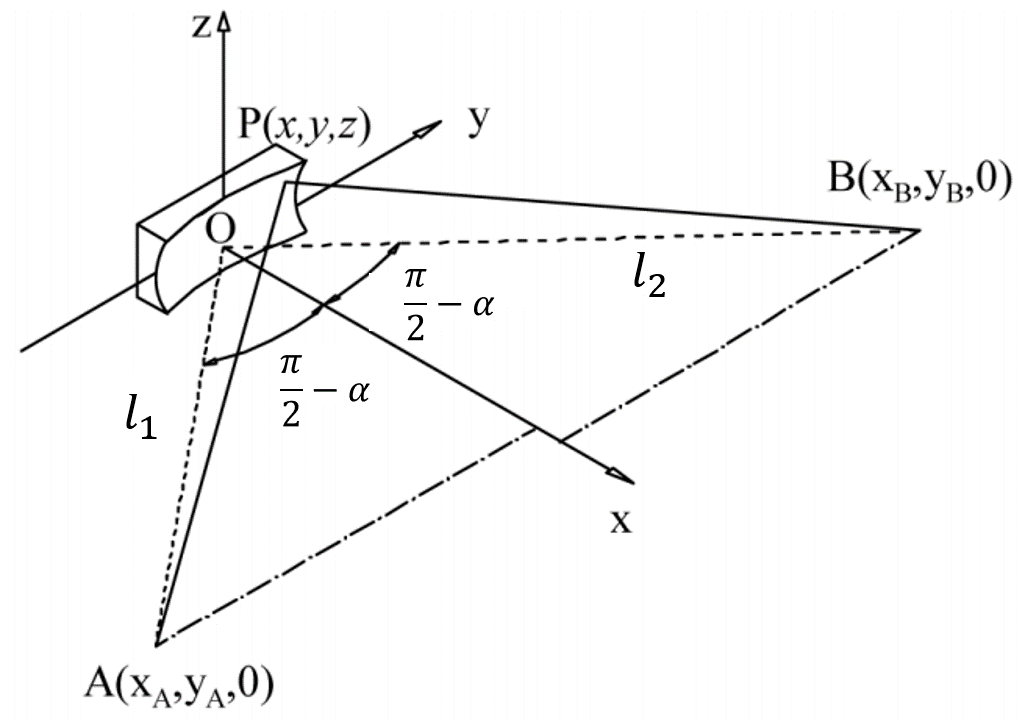
\includegraphics[width=0.75\textwidth]{figures/chap2/TM_geometry.png}
	\caption{placeholder text.}
	\label{fig:TM_geometry}
	% credit the image source here
\end{figure}

\begin{figure}
	\centering
	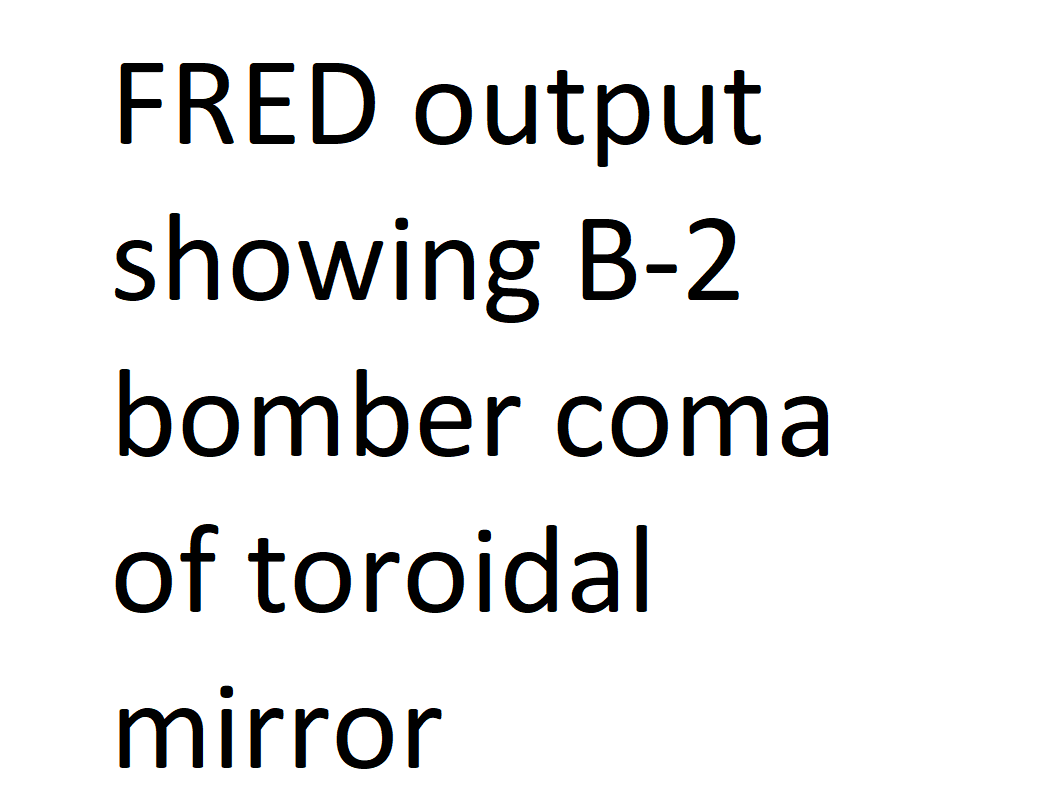
\includegraphics[width=0.75\textwidth]{figures/chap2/TM_coma.png}
	\caption{placeholder text.}
	\label{fig:TM_coma}
	% credit the image source here
\end{figure}

geometric description of toroidal mirror, including equations / parameters

\begin{align}
\frac{1}{r} + \frac{1}{r'} &= \frac{2}{R \cos \alpha} \\
\frac{1}{r} + \frac{1}{r'} &= \frac{2 \cos \alpha}{\rho}
\end{align}

\begin{align}
f_t &= \frac{1}{2} R \cos \alpha \\
f_s &= \frac{1}{2} \frac{\rho}{\cos \alpha}
\end{align}

setting $f_t = f_s$, we obtain $r/R = \cos^2 \alpha$.

\begin{equation}
\Delta y^{'}_{lc} = \frac{1}{2} \frac{l^2 \sin \alpha}{\rho} (M-1)
\end{equation}

where $M=r/r'$ is the magnification.

figure showing geometry

equal path length equations - choosing the optimal source, focal positions

coma and aberration when magnification is not unity

multi-mirror configurations (avoided due to complexity, size)

\subsubsection{ellipsoidal mirrors}

geometric description, including equations. what parameters describe this optic?

figure showing geometry

coma and aberration are not an issue - why not?

advantage: single-mirror configuration

disadvantage: difficulty in manufacturing a non-spherical / non-cylindrical surface. solution: active


\subsection{entrance and exit arm length choice}
2250 mm entrance, 750 mm exit arm.

due to the modular nature of the beamline, we were limited on how short the exit arm could be. given the chamber geometries and the placement of the recombination optic, the exit arm had to be at least 750 mm. 

\subsection{mirror physical dimensions choice}
this had to do with the assumed divergence of the XUV light and the entrance arm length.

\subsection{ellipsoid mirror math}
\begin{figure}
	\centering
	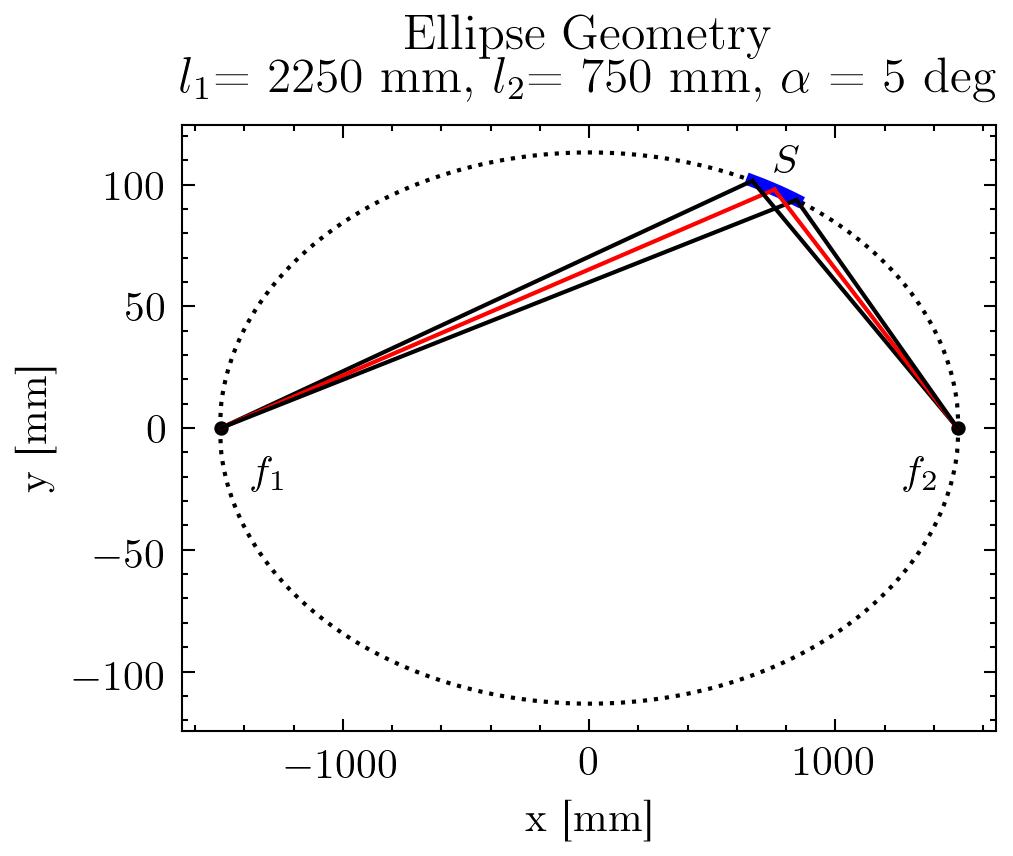
\includegraphics[width=0.75\textwidth]{figures/chap2/EM_2D.png}
	\caption{Overhead view of the ellipsoidal mirror geometry. Mirror surface $S$ is shown in blue; foci $f_{1,2}$ are represented by black dots. Rays that strike the center (red) and the edges (black) of the mirror are depicted as lines. Vertical scale is enlarged to show detail.}
	\label{fig:EM_2D}
	% figure made in EM_geometry.py
\end{figure}

\begin{figure}
	\centering
	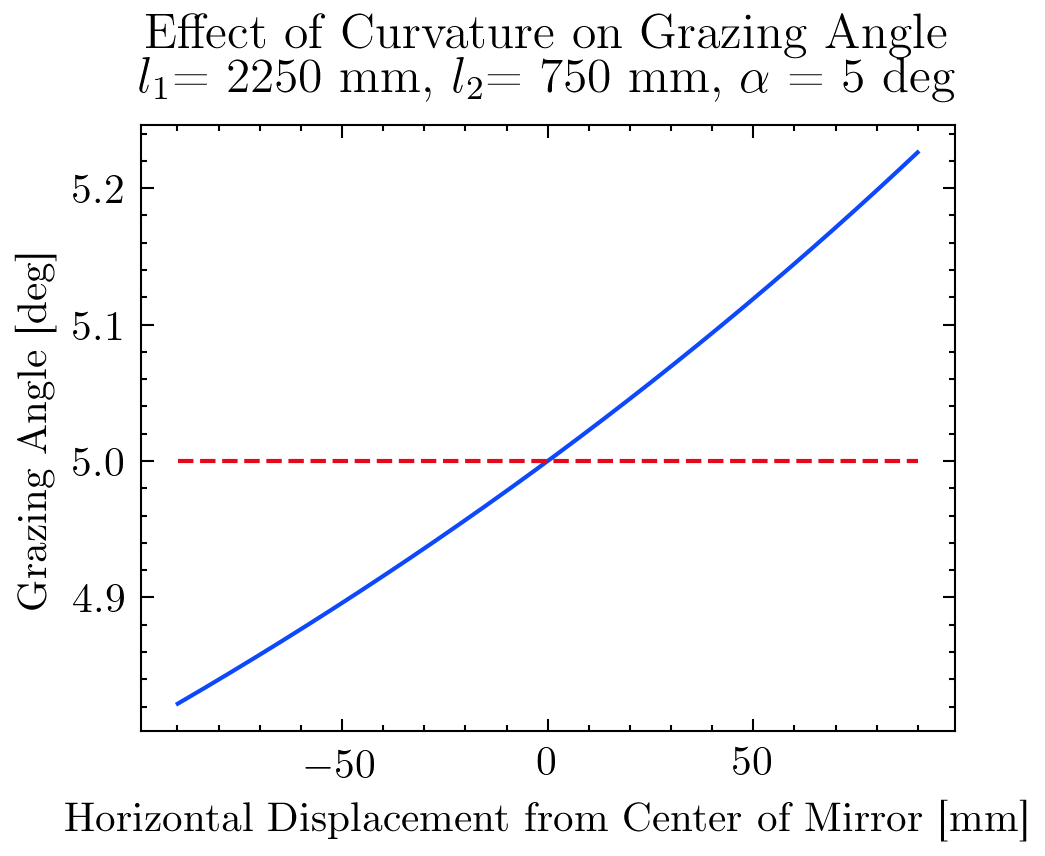
\includegraphics[width=0.75\textwidth]{figures/chap2/EM_angle.png}
	\caption{The effect of curvature on the local grazing angle. Light that strikes the edges of the mirror will experience a slightly different grazing angle than the design angle.}
	\label{fig:EM_angle}
	% figure made in EM_geometry.py
\end{figure}

\begin{figure}
	\centering
	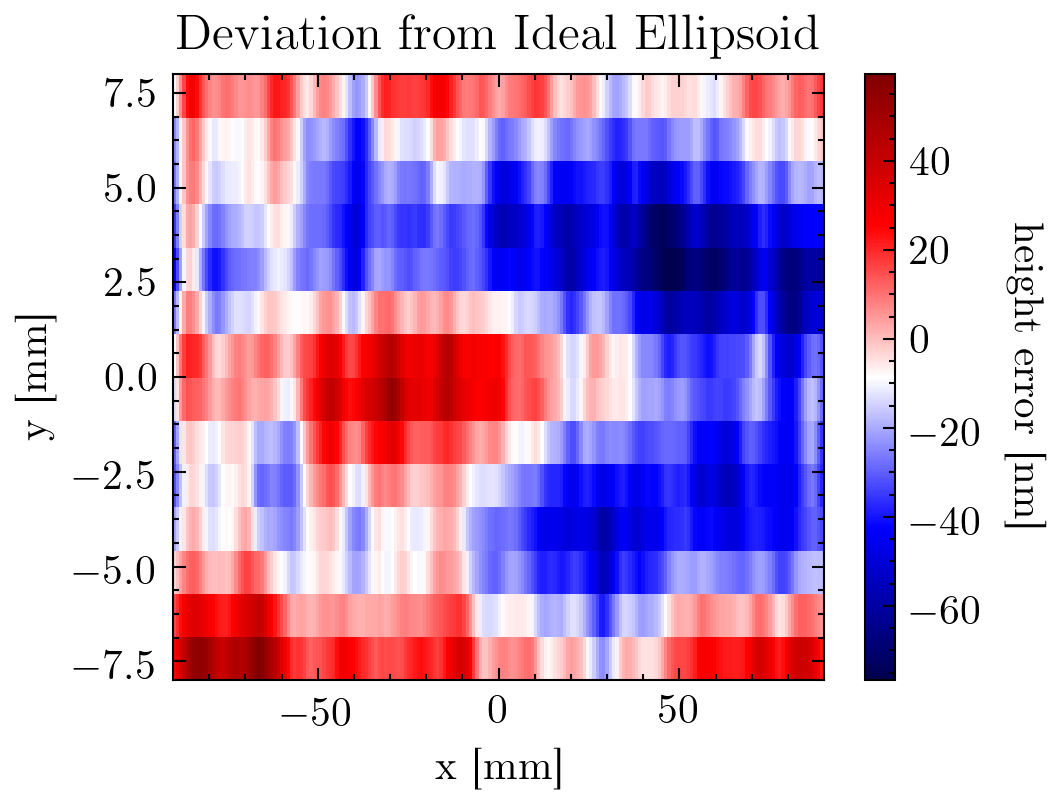
\includegraphics[width=0.75\textwidth]{figures/chap2/EM_error.png}
	\caption{Data provided by Carl Zeiss Laser Optics GmbH.}
	\label{fig:EM_error}
	% figure made in EM_geometry.py. data obtained from private communication with Norman Niewrzella of Zeiss. 
\end{figure}

The surface of an ellipsoidal mirror is a section of an ellipsoid of revolution. In a Cartesian coordinate system, an ellipsoid of revolution is described by parameters $a$ and $b$:
\begin{equation}
\frac{x^2}{a^2} + \frac{y^2 + z^2}{b^2} = 1
\end{equation}
where the $xy$ plane is the optical plane and $z$ is the vertical direction. Due to the symmetry between $y$ and $z$, much of the analysis can be done on a two-dimensional ellipse:
\begin{equation}
\frac{x^2}{a^2} + \frac{y^2}{b^2} = 1
\label{eqn:ellipse}
\end{equation}
In the $xy$ plane, the surface of the mirror is a segment of the curve formed by \cref{eqn:ellipse}. The center of the mirror is centered at position $(x,y)=(x_M, y_M)$. The ellipse has eccentricity $\epsilon$,
\begin{equation}
\epsilon = \sqrt{1-\frac{b^2}{a^2} } \text{,}
\end{equation}
and focal points at positions $(x,y) = (\pm a \epsilon,0)$. Consider a light source at the first focal point,  $f_1 = (-a \epsilon,0)$: rays emanating from $f_1$ will strike surface of the ellipse at some point $S = (x_0, y_0)$ and focus to $f_2 = (a \epsilon,0)$. This geometry is shown in \cref{fig:EM_2D}. This optical system has an entrance arm $l_1 = f_1S$, exit arm $l_2=Sf_1$, and demagnification $M$ given by:
\begin{align}
l_1(x_0, y_0) &= \sqrt{ (x_0+a \epsilon)^2 + y_0^2 } \\
l_2(x_0, y_0) &= \sqrt{ (x_0-a \epsilon)^2 + y_0^2 } \\
M &= \frac{l_1}{l_2}
\end{align}
Once the $f_1$, $f_2$ and $S$ are defined, the grazing angle $\alpha$ of reflection can be found by applying the Law of Cosines:
\begin{equation}
\alpha = \frac{1}{2} \arccos \left( \frac{(2 a \epsilon)^2 - l_1^2 - l_2^2}{2 l_1 l_2} \right)
\end{equation}
The finite spatial extent of a physical mirror will result in a range of grazing angles across the surface of the mirror. The grazing angle for our mirror is shown in \cref{fig:EM_angle}. The curvature of the ellipsoidal mirror is characterized by three parameters: the semi-major axis $a$, semi-minor axis $b$, and off-axis position $x_M$, or equivalently by the entrance arm $l_1$, exit arm $l_2$ and grazing angle $\alpha$. Additionally, the spatial extent (clear aperture) of the mirror must be specified by the tangential length $L$ and the out-of-plane width $W$.



The problem with an adhesion layer is that over time it diffuses to the surface, so eventually you may observe Cr lines in your spectrum.  However, without the adhesion layer the Au film is quite fragile.  


The actual roughness-values will be somewhere between 0.3 and 5nm RMS, degrading to the edge.



\section{HHG Gas Source}

Transient absorption experiments require a high XUV photon flux for a variety of reasons. First, the sample thickness is usually chosen such that the XUV transmission is roughly 50\% near the spectral feature of interest. This optical density represents a compromise between the incompatible goals of having a strong ground state absorption (which allows you to easily detect small changes in optical density) while simultaneously avoiding the noise floor of the detector (which is required for good statistics). As a result, half of the XUV photons will never reach the detector, so you better be making a lot of them. Second, a high XUV flux will reduce the number of laser shots required for a given data point, which in turn reduces the chances of inadvertently damaging your sample with the infrared laser. Finally, a high flux reduces the overall time required to complete an experiment. Besides the obvious benefit of happier graduate students, the ability to quickly perform an experiment increases data fidelity by reducing the effects of unavoidable experimental noise sources such as long-term laser drift (either pointing or energy) or environmental changes caused by the building's HVAC system.

Depending on the energy of the spectral feature, obtaining a high photon flux can range from trivial to challenging. There are many (usually interdependent) experimental parameters (gas type, interaction pressure and length, wavelength, intensity, confocal parameter, focal position relative to gas source, etc.) that can be tuned to optimize photon flux. Physically, these parameters can change the microscopic single atom response, the macroscopic coherent addition of dipole emitters (via phase matching), or both. Each experiment will usually require a unique combination of experimental settings to achieve a usable light source. For example, optimizing the harmonic yield at 100 eV for a Si L-edge measurement will usually come at the expense of harmonics yield in the 30-50 eV range, which are used to measure the transition metal M-edges.

In general, an experimentalist has neither perfect knowledge nor control over all the variables that contribute towards phase matching. Setting aside the complicated topic of phase matching, the one dimensional on-axis phase matching model\cite{constantOptimizingHighHarmonic1999} shows that the photon flux is proportional to the square of the pressure-length product of the interaction gas. That is, so long as we can remain phase matched and below the critical phase matching pressure\cite{popmintchevPhaseMatchingHigh2009}, we can universally increase the harmonic flux of our experiments by increasing the pressure-length product.

Unfortunately, one cannot ignore phase matching. Oftentimes, the spectral feature of interest lies beyond the harmonic cutoff when using the more convenient shorter wavelengths. In this case, the fundamental wavelength is increased to extend the cutoff (which scales as $\lambda^2$). However, the critical phase matching pressure also scales as $\lambda^2$ \cite{popmintchevPhaseMatchingHigh2009}, and the single atom response scales as $\lambda^{-(5-6)}$ \cite{tateScalingWavePacketDynamics2007}. These two combined effects result in a dramatically decreased photon flux if intensity and pressure are kept constant with increasing wavelength, often to the point that the resulting flux is insufficient for a transient absorption experiment, even though your cutoff has been extended to the proper energy. While some of the flux can be recovered by increasing the backing pressure of the continuous free expansion nozzle, the generation chamber's finite pumping speed limits the efficacy of pressure tuning at the longer wavelengths. Even at 800 nm, the maximum backing pressure of the continuous free expansion nozzle results in an interaction pressure below the critical phase matching pressure. Practically speaking, the continuous free expansion gas nozzle is not suitable for transient absorption experiments using the signal wavelengths ($\lambda > 1.6 \ \mu m$) or with spectral features greater than the aluminum edge at 72 eV.

Providing the lab with a brighter harmonic source was the ultimate goal of the high pressure cell, and for the most part this goal was achieved. Below, we will review the basic design considerations, drawbacks and advantages of the three main types of gas sources used in this thesis: the free expansion nozzle, the low pressure cell and the high pressure cell. A primer on how to install and use the high pressure cell can be found in Appendix \ref{appendix:TABLe_manual}.

\subsection{Continuous Free Expansion Nozzle}
%outline of gas jet physics:
%- why supersonic? basic physics argument
%- outline of derivation to get to the T/P/rho relationships
%- outline of derivation to get to the centerline equations
%- mach disk location, description, thickness
%- derivation of gas nozzle throughput T
%
\begin{figure}
	\centering
	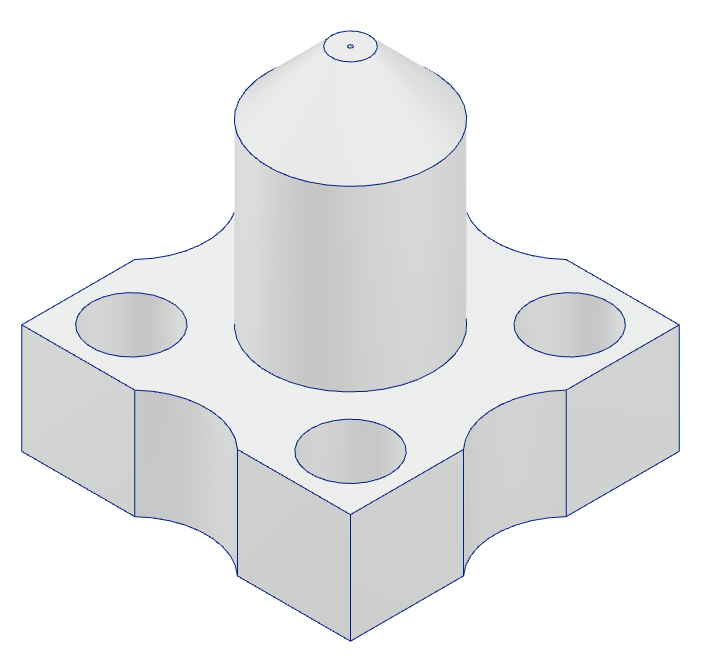
\includegraphics[width=0.5\textwidth]{figures/chap2/gas_nozzle.png}
	\caption{The continuous free expansion nozzle. Gas flows from the base of the nozzle and out of the 200 $\mu$m aperture. The large through holes on the base of the nozzle are for mounting to the gas delivery system; the sidewall cuts are for clearance for other mounting hardware. The top surface is beveled to reduce the minimum allowable distance between the laser axis and the nozzle.}
	\label{fig:gas_nozzle}
\end{figure}

\begin{figure}
	\centering
	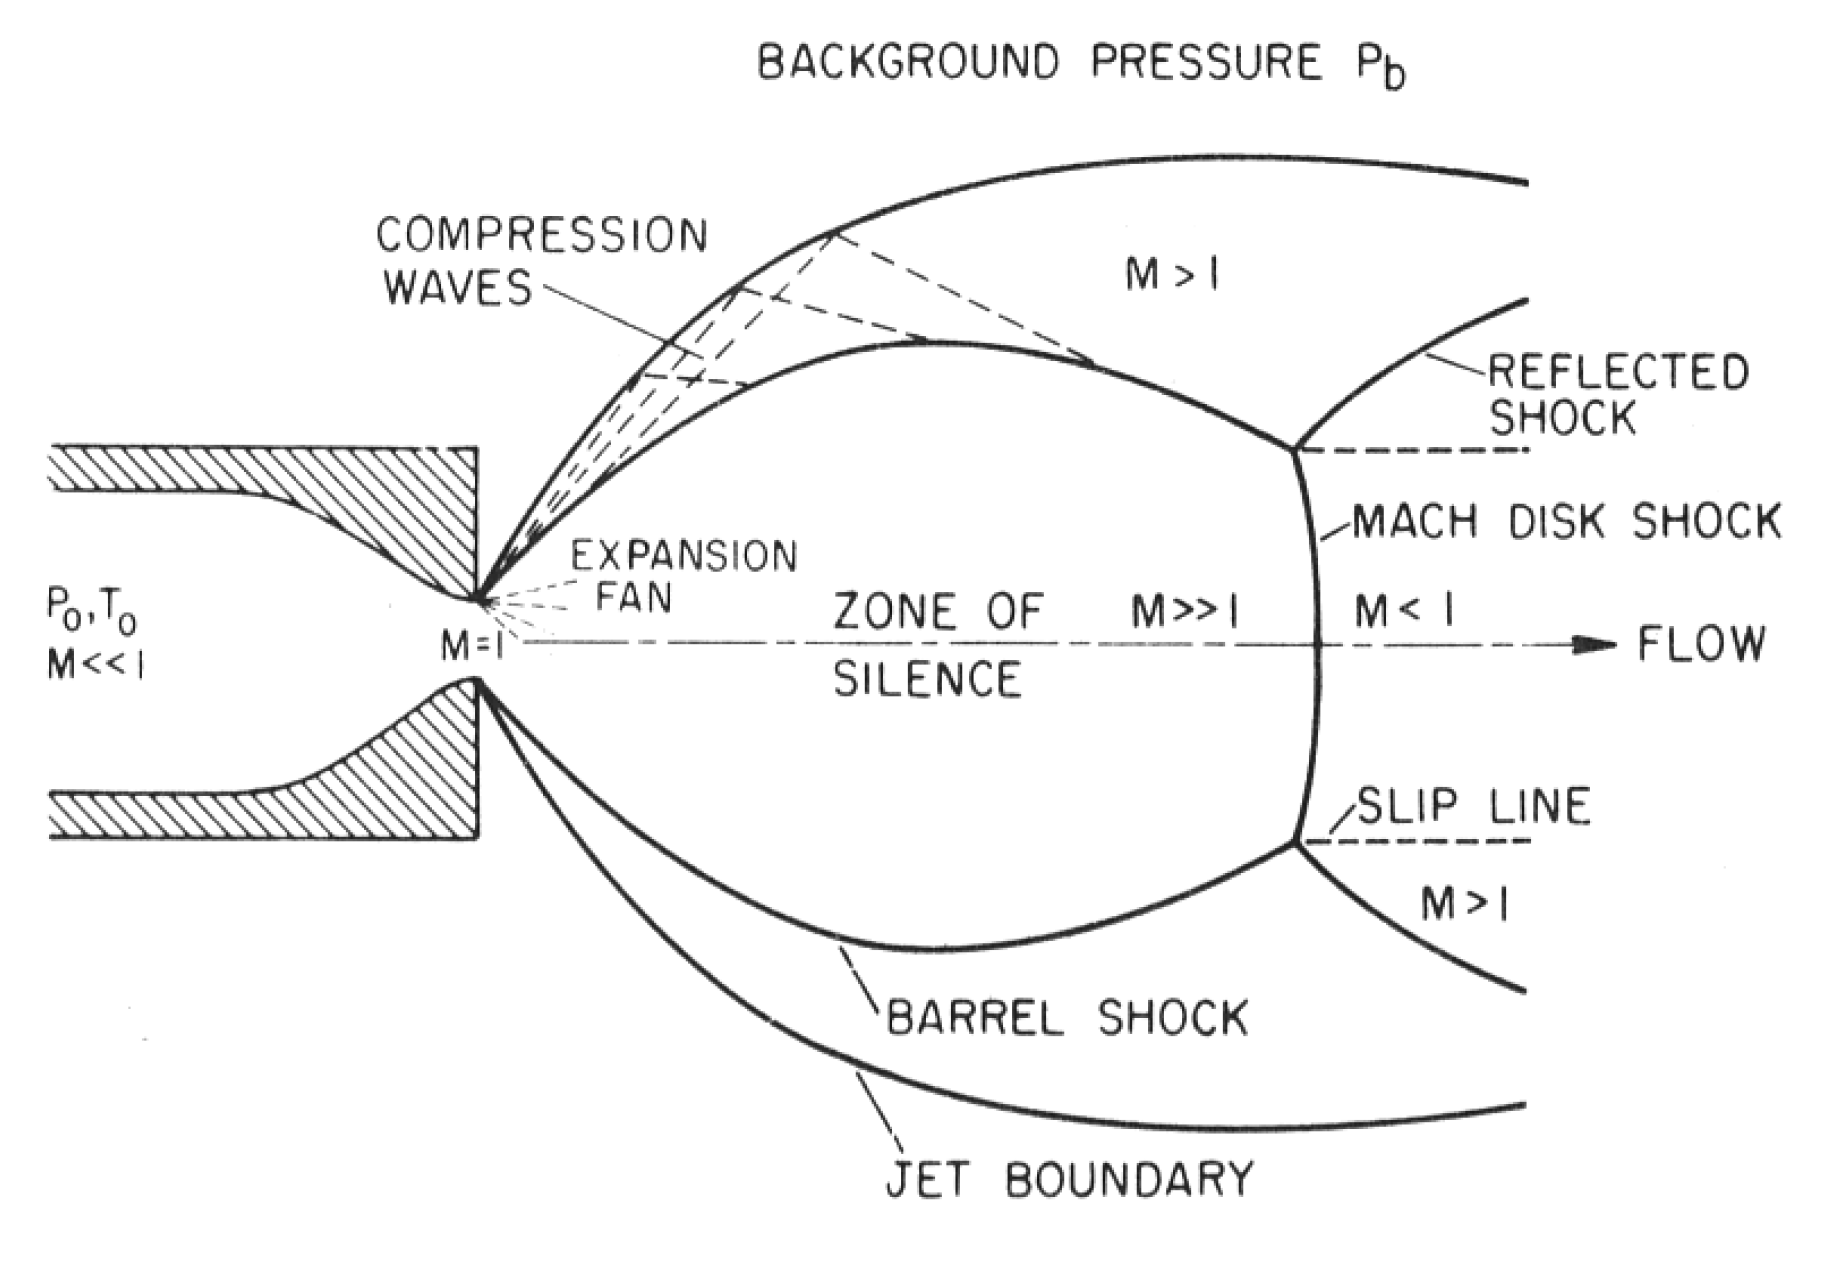
\includegraphics[width=0.5\textwidth]{figures/chap2/gas_expansion.PNG}
	\caption{The structure of the supersonic gas plume after leaving a gas nozzle. This figure was taken from Ref \cite{millerFreeJetSources1988}.}
	\label{fig:gas_expansion}
\end{figure}

\begin{figure}
	\centering
	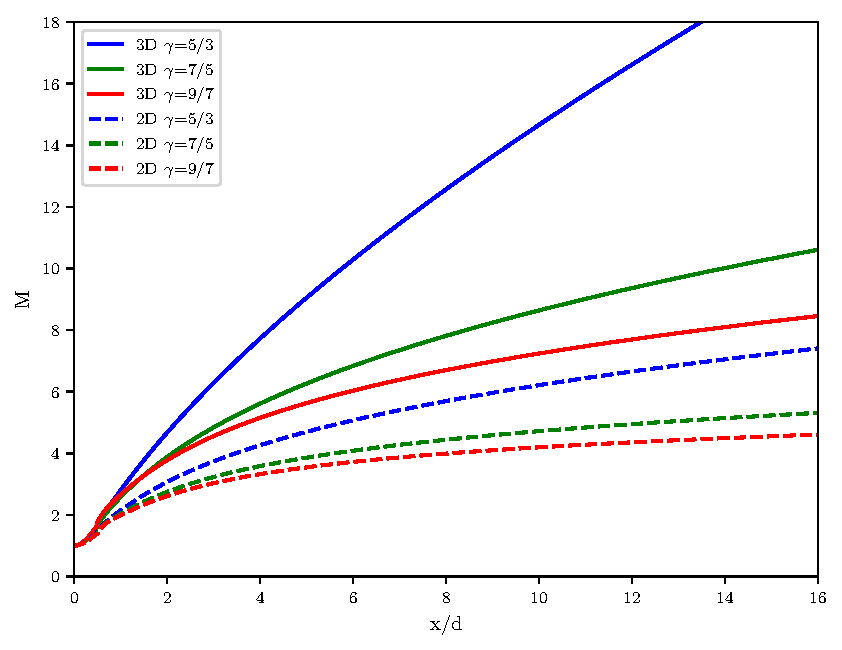
\includegraphics{figures/chap2/Scoles_Fig25.pdf}
	\caption{Centerline Mach number versus distance in nozzle diameters for 2D (planar) and 3D (axisymmetric) geometries, calculated using \cref{eqn:Scoles_centerline2.2}.}
	\label{fig:scoles_mach}
\end{figure}

\begin{figure}
	\centering
	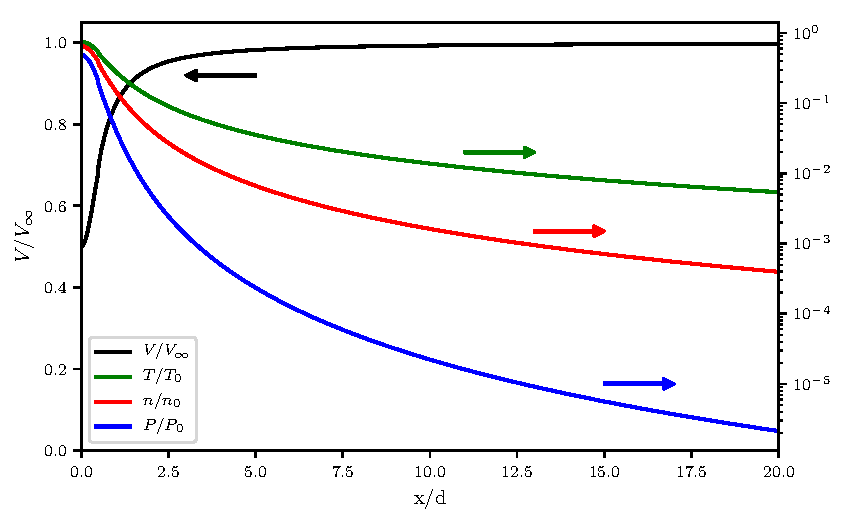
\includegraphics{figures/chap2/Scoles_Fig23.pdf}
	\caption{Free jet centerline properties versus distance in nozzle diameters for helium gas ($\gamma$=5/3, W=4). Mach number is calculated using \cref{eqn:Scoles_centerline2.2}, and the centerline properties are calculated using \cref{eqn:mach_properties}. Velocity $V$ is scaled by terminal velocity $V_{\infty}$; temperature $T$, number density $n$ and pressure $P$ are normalized by source stagnation values $T_0$, $n_0$, $P_0$.}
	\label{fig:scoles_centerline}
\end{figure}

When gas flows from a high pressure region ($P_0$) to a low pressure region ($P_b$) through a small aperture, a plume will form in the low pressure region. If the pressure ratio $P_0/P_b$ exceeds a critical value $G \equiv ((\gamma+1)/2)^{\gamma/(\gamma-1)}$, then the gas flow may exceed the local speed of sound. This critical value is at most 2.1 for all gases, so we easily exceed it in all of our experiments.\footnote{The highest chamber pressures in our experiments are on the order of $P_b \approx 10$ mTorr. Therefore, any nozzle that is backed by more than $P_0 \approx 21$ mTorr will result in a supersonic gas flow. Typical backing pressures for harmonic generation are on the order of 250 Torr, putting us well within the supersonic regime.} It is therefore necessary to understand the basic properties of supersonic gas plumes.

The continuous free expansion nozzle consists of a small diameter hole drilled in a block of aluminum, shaped to be convenient for gas delivery and assembly.\footnote{To reduce the gas load on the pumps, we used $200 \ \mu m$ diameter nozzles. This was the smallest size hole the machine shop could readily drill into aluminum.} The basic design is shown in \cref{fig:gas_nozzle}. The structure of the resulting supersonic plume is shown in \cref{fig:gas_expansion}. The physics of supersonic gas flow has been extensively studied in the literature and will not be discussed at length here. Below is a brief overview of the relevant physics required to understand the gas nozzles used for HHG in our lab. For a more detailed review of the field, see Ref \cite{millerFreeJetSources1988}.

% derivation of \cref{eqn:gas_dens}
energy equation. $V$ is velocity, $h$ is enthalpy per unit mass.
\begin{equation}
h + V^2/2 = h_0
\end{equation}
for ideal gases, $dh = \hat{C}_p \ dt$, and we have

\begin{equation}
V^2 = 2(h_0 -h) = 2 \int_{T}^{T_0} \hat{C}_p \ dT
\label{eqn:Scoles_gas_jet_energy}
\end{equation}

For an ideal gas, $\hat{C}_p = \gamma / (\gamma-1) (R/W)$, where $\gamma = C_p/C_V$ is the ratio of the specific heats, $R$ is the gas constant, $W$ is the molecular weight. if the gas is cooled substantially in the expansion ($T \ll T_0$), then we have:

\begin{equation}
V_{\infty} = \sqrt{ \frac{2R}{W} \left( \frac{\gamma}{\gamma-1} \right) T_0 }
\end{equation}

For an ideal gas, the speed of sound is $a = \sqrt{\gamma R T/W}$ and the Mach number is $M = V/a$. Assuming $\hat{C}_p$ is constant, we can recast \cref{eqn:Scoles_gas_jet_energy} in terms of $\gamma$ and $M$.  Using these assumptions, one can obtain the following relationships for the temperature $T$, velocity $V$, pressure $P$, mass density $\rho$ and number density $n$ in the gas jet scaled to those parameters at the stagnation point $(T_0, P_0, \rho_0, n_0)$:

\begin{subequations}
\label{eqn:mach_properties}
\begin{align}
	% eqn 2.3 - 2.6 in scoles, page 18
(T/T_0) &= \left(  1 + \frac{\gamma-1}{2} M^2 \right)^{-1} \label{eqn:gas_temp} \\
V &= M \sqrt{ \frac{\gamma R T_0}{W} } \left( 1 + \frac{\gamma-1}{2} M^2 \right)^{-1/2} \label{eqn:gas_velo} \\
(P/P_0) &= (T/T_0)^{\gamma/(\gamma-1)} = \left(  1 + \frac{\gamma-1}{2} M^2 \right)^{-\gamma/(\gamma-1)} \label{eqn:gas_pres} \\
(\rho/\rho_0) &= (n/n_0) = (T/T_0)^{1/(\gamma-1)} = \left(  1 + \frac{\gamma-1}{2} M^2 \right)^{-1/(\gamma-1)} \label{eqn:gas_dens}
\end{align}
\end{subequations}

Therefore, once we know the Mach number $M$, we can calculate the above properties for the gas jet. The Mach number is found by solving the fluid mechanics equations dealing with the conversation of mass, momentum and energy:

\begin{subequations}
\label{eqn:scoles_continuum}
\begin{flalign}
% eqn 2.7 of scoles, page 19
\text{mass:} && \nabla \cdot (\rho \mathbf{V}) &= 0 && \label{eqn:scoles_mass} \\
\text{momentum:} && \rho \mathbf{V} \cdot \nabla \mathbf{V} &= - \nabla P  && \label{eqn:scoles_momentum} \\
\text{energy:} && \mathbf{V} \cdot \nabla h_0 &= 0 \textrm{ or } h_0 = \textrm{constant along streamlines} \label{eqn:scoles_energy} && \\
\text{equation of state:} && P &= \rho \frac{R}{W} T  && \label{eqn:scoles_eqn-state} \\
\text{thermal equation of state:} && dh &= \hat{C}_P \ dT \label{eqn:scoles_thermal-eqn-state} && 
\end{flalign}
\end{subequations}

The above equations are valid for an isentropic, compressible flow of a single component ideal gas molecular weight $W$ and constant specific heat ratio $\gamma$. A steady state is assumed and viscosity and heat conduction are neglected. These equations have been numerically solved in the literature for two source geometries: a ``slit" nozzle (2D, planar) and a circular aperture (3D, axisymmetric). The numerical solutions to each geometry scale with the nozzle diameter $d$, and have been fit to the following analytical functions:

\begin{subequations}
	\label{eqn:Scoles_centerline2.2}
	\begin{align}
	% eqns from table 2.2 of scoles, page 23
	\frac{x}{d} > 0.5&: &&M = \left( \frac{x}{d} \right)^{(\gamma-1)/j} \left[ C_1 + \frac{C_2}{\left(\frac{x}{d}\right)} + \frac{C_3}{\left(\frac{x}{d}\right)^2} + \frac{C_4}{\left(\frac{x}{d}\right)^3} \right] \label{eqn:Scoles_centerline1} \\
	0 < \frac{x}{d} < 1.0&: &&M = 1.0 + A \left( \frac{x}{d} \right)^2 + B \left( \frac{x}{d} \right)^3 \label{eqn:Scoles_centerline2}
	\end{align}
\end{subequations}

\textbf{question: why does M increase without bound with increasing x, while V is limited to a finite value? scoles has a discussion, you should address it here.}

The fitting coefficients for \cref{eqn:Scoles_centerline2.2} are listed in \cref{tbl:Scoles_gas_params2.2}. A plot of the results for different source geometries and gases are shown in \cref{fig:scoles_mach}.


\begin{table}[]
	\centering
	\begin{tabular}{lllllllll}
		\hline
		\multicolumn{1}{c}{Source} & \multicolumn{1}{c}{$j$} & \multicolumn{1}{c}{$\gamma$} & \multicolumn{1}{c}{$C_1$} & \multicolumn{1}{c}{$C_2$} & \multicolumn{1}{c}{$C_3$} & \multicolumn{1}{c}{$C_4$} & \multicolumn{1}{c}{$A$} & \multicolumn{1}{c}{$B$} \\ \hline
		3D                         & 1                     & 5/3                          & 3.232                     & -0.7563                   & 0.3937                    & -0.0729                   & 3.337                & -1.541                \\
		3D                         & 1                     & 7/5                          & 3.606                     & -1.742                    & 0.9226                    & -0.2069                   & 3.190                 & -1.610                \\
		3D                         & 1                     & 9/7                          & 3.971                     & -2.327                    & 1.326                     & -0.311                    & 3.609                 & -1.950                \\
		2D                         & 2                     & 5/3                          & 3.038                     & -1.629                    & 0.9587                    & -0.2229                   & 2.339                 & -1.194                \\
		2D                         & 2                     & 7/5                          & 3.185                     & -2.195                    & 1.391                     & -0.3436                   & 2.261                 & -1.224                \\
		2D                         & 2                     & 9/7                          & 3.252                     & -2.473                    & 1.616                     & -0.4068                   & 2.219                 & -1.231               
	\end{tabular}
\caption{Gas parameters used in free expansion calculations, with \cref{eqn:Scoles_centerline2.2}. Table recreated from Ref \cite{millerFreeJetSources1988}.}
\label{tbl:Scoles_gas_params2.2}
\end{table}


\cref{tbl:Scoles_mach_params} shows the centerline Mach numbers used in the following equations:

\begin{subequations}
	\label{eqn:Scoles_centerline2.1}
	% eqns from table 2.1 of scoles, page 22
	\begin{align}
		M &= A \left( \frac{x-x_0}{d}\right)^{\gamma-1} - \frac{\frac{1}{2} \left( \frac{\gamma+1}{\gamma-1} \right)}{A \left(\frac{x-x_0}{d} \right)^{\gamma-1}} \label{eqn:gas_mach} \\
		\frac{\rho(y,x)}{\rho(0,x)} &= \cos^2(\theta) \cos^2\left(\frac{\pi\theta}{2\phi}\right) \\
		\frac{\rho(R,\theta)}{\rho(R,0)} &= \cos^2\left(\frac{\pi\theta}{2\phi}\right) \\
		\left(\frac{x}{d} \right) &> \left( \frac{x}{d} \right)_{\text{min}} \label{eqn:mach_cond}
	\end{align}
\end{subequations}
The gas nozzle throughput $\hat{T}$ is calculated from:


\begin{equation}
\hat{T} \ (\text{torr} \cdot \text{l}/\text{s}) = \hat{S} \cdot P_b = C \left(\frac{T_C}{T_0} \right)\sqrt{\frac{300}{T_0}}(P_0 d) d
\label{eqn:nozzle_thruput}
\end{equation}

where $C$ is the gas constant from \cref{tbl:Scoles_gas_params}, $P_0$ is the nozzle's backing pressure in Torr, $T_C$ and $T_0$ are the vacuum chamber and backing temperatures, respectively, in Kelvin, $P_0$ is the backing pressure in Torr, and $d$ is the nozzle's diameter in cm.

S = pumping speed?
Pb = chamber pressure

(how was this equation derived?)

Note that the gas nozzle throughput is proportional to both backing pressure and diameter of the nozzle. For our vacuum system, the generation chamber has a pumping speed of approximately ???; 

Relevant gas parameters are listed in \cref{tbl:Scoles_gas_params}.

condition for supersonic flow: the pressure ratio $P_0 / P_b$ exceeds a critical value $G \equiv ((\gamma+1)/2)^{\gamma/(\gamma-1)}$, which is less than 2.1 for all gases. Since the vacuum chamber pressure is at most 10 mTorr, just about any backing pressure will result in supersonic flow out of the gas nozzle.

Mach disk location: $x_M / d = 0.67(P_0/P_b)^{1/2}$. for example, for a chamber pressure of 10 mTorr and a backing pressure of -5 psig ($\sim$450 Torr), the Mach disk is located about 45 nozzle diameters away from the orifice. for a 200 micron diameter nozzle, that's about 9 cm.

\begin{table}[]
	\centering
	\begin{tabular}{llllll}
		Gas    & $\epsilon / k$ (K) & $\sigma$ (angstrom) & $C_6 / k$ ($10^{-43}$ K $\cdot$ cm$^6$) & $Z_r$     & \begin{tabular}[c]{@{}l@{}}C (l/cm$^2$/s);\\ \cref{eqn:nozzle_thruput}\end{tabular} \\ \hline
		He     & 10.9               & 2.66                & 0.154                                   & -         & 45                                                               \\
		Ne     & 43.8               & 2.75                & 0.758                                   & -         & 20                                                               \\
		Ar     & 144.4              & 3.33                & 7.88                                    & -         & 14                                                               \\
		Kr     & 190                & 3.59                & 16.3                                    & -         & 9.8                                                              \\
		Xe     & 163                & 4.3                 & 41.2                                    & -         & 7.9                                                              \\
		H$_2$  & 39.6               & 2.76                & 0.7                                     & $\sim$300 & 60-63                                                            \\
		D$_2$  & 35.2               & 2.95                & 0.93                                    & $\sim$200 & 42                                                               \\
		N$_2$  & 47.6               & 3.85                & 6.2                                     & $\sim$2.5 & 16                                                               \\
		CO     & 32.8               & 3.92                & 4.76                                    & $\sim$4.5 & 16                                                               \\
		CO$_2$ & 190                & 4.0                 & 31.1                                    & $\sim$2.5 & 12-13                                                            \\
		CH$_4$ & 148                & 3.81                & 18.1                                    & $\sim$15  & 21                                                               \\
		O$_2$  & 115                & 3.49                & 8.31                                    & $\sim$2   & 15                                                               \\
		F$_2$  & 121                & 3.6                 & 10.5                                    & $\sim$3.5 & 14                                                               \\
		I$_2$  & 550                & 4.98                & 336                                     & $\sim$1   & 5.2                                                              \\ \hline
	\end{tabular}
\caption{Gas parameters used in free expansion calculations. Table recreated from Ref \cite{millerFreeJetSources1988}.}
\label{tbl:Scoles_gas_params2.1}
\end{table}

\begin{table}[]
	\centering
	\begin{tabular}{lllll}
		\hline
		$\gamma$ & $x_0/d$ & $A$  & $\phi$ & $(x/d)_{\text{min}}$ \\ \hline
		1.67     & 0.075   & 3.26 & 1.365  & 2.5                  \\
		1.40     & 0.4     & 3.65 & 1.662  & 6                    \\
		1.2857   & 0.85    & 3.96 & 1.888  & 4                    \\
		1.20     & 1.00    & 4.29 & -      & -                    \\
		1.10     & 1.60    & 5.25 & -      & -                    \\
		1.05     & 1.80    & 6.44 & -      & -                    \\ \hline
	\end{tabular}
\caption{Centerline Mach Number and Off-Axis Density Correlations for Axisymmetric Flow. Table recreated from Ref \cite{millerFreeJetSources1988}.}
\label{tbl:Scoles_mach_params}
\end{table}

basic design of free expansion nozzle

throughput calculations (Scoles)

harmonic yield results

note: i did not design this cell

advantages: easy to align, cheap to produce, free-expansion cooling (for alignment experiments)

disadvantages: small pressure length product. very low interaction pressure. impossible to phase match longer wavelengths. overall low yield. 

\subsection{low pressure cell}

\begin{figure}
	\centering
	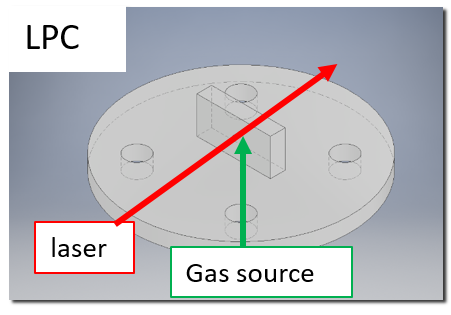
\includegraphics[width=0.5\textwidth]{figures/chap2/LPC_diagram.png}
	\caption{Detail of the LPC interaction region.}
	\label{fig:LPC_diagram}
\end{figure}

\begin{figure}
	\centering
	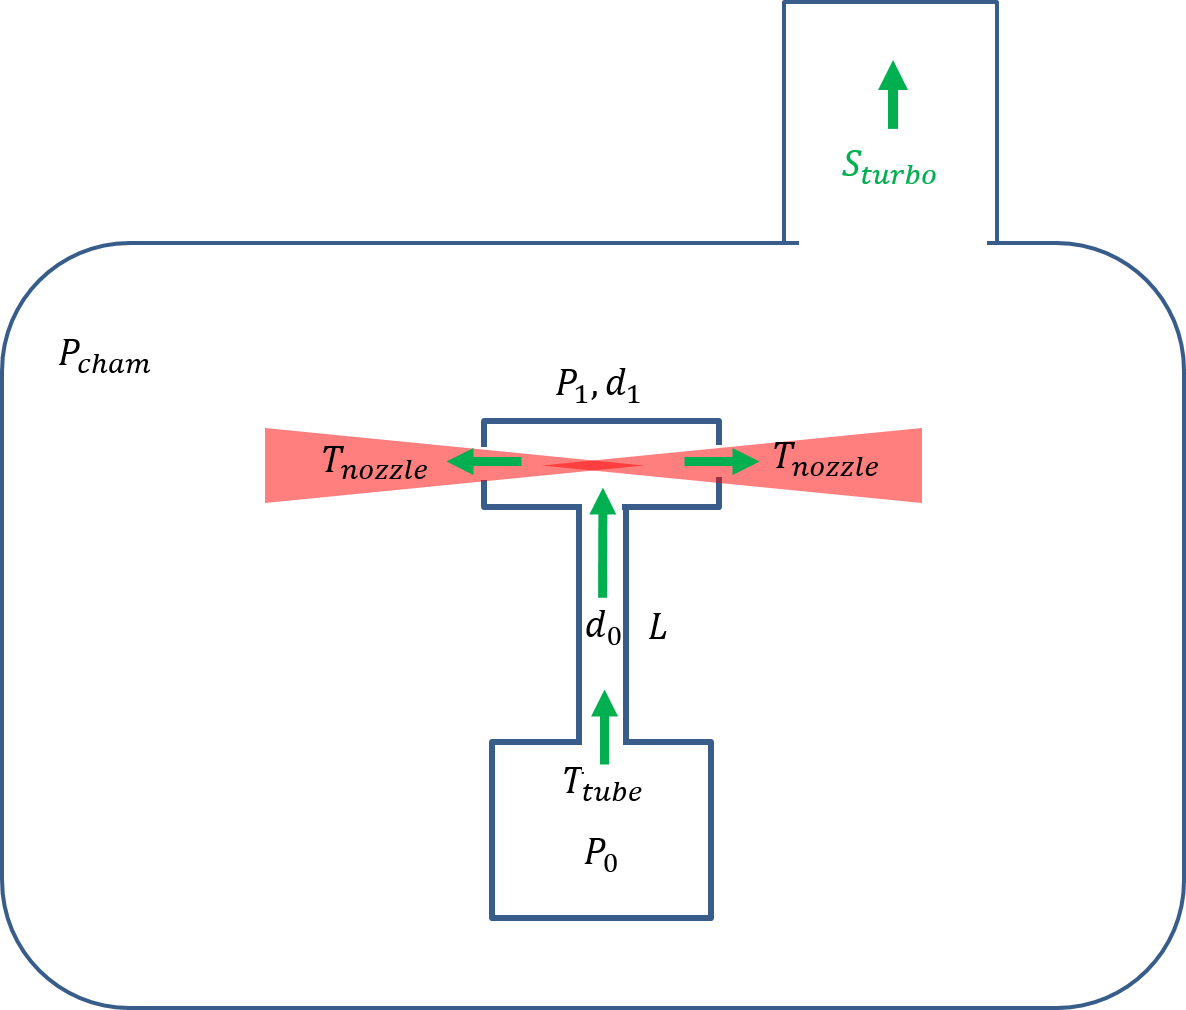
\includegraphics[width=0.75\textwidth]{figures/chap2/LPC_schematic2.png}
	\caption{Gas flow schematic of the LPC. The green arrows indicate the direction of gas flow, and the red shaded region indicates the laser path. An infinite reservoir of gas with backing pressure $P_0$ supplies the laser interaction region with gas via a thin capillary of diameter $d_0$, length $L$ and throughput $T_{tube}$. The interaction region has pressure $P_1$ and diameter $d_1$. The interaction region acts as a pressure source for two diametrically opposed supersonic gas jets, each with throughput $T_{nozzle}$. The generation chamber has a turbopump with pumping speed $S_{turbo}$ and an equilibrium pressure $P_{cham}$.}
	\label{fig:LPC_schematic}
\end{figure}

basic design of low pressure cell -- gas load, Rayleigh range, spot size, laser drift

gas load calculations (simple model)

harmonic yield results

note that i did not design this cell. design is from (now Dr.) Zhou Wang.

advantages: increased interaction length - brighter! easy to align.

disadvantages: relative to the free expansion nozzle, you don't get any cooling.

\subsection{high pressure cell}

\begin{figure}
	\centering
	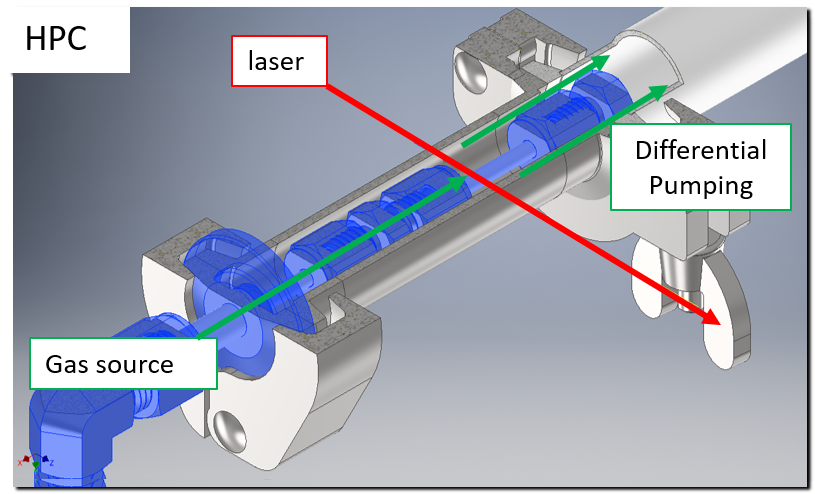
\includegraphics[width=0.9\textwidth]{figures/chap2/HPC_cutaway2.png}
	\caption{Detail of the HPC interaction region. From bottom left to top right: welded gas feedthrough, concentric inner \& outer pipes, edge-welded bellows. The high pressure region is shaded blue. The green lines indicate the gas flow direction; the red line indicates the laser propagation direction.}
	\label{fig:HPC_cutaway2}
\end{figure}

\begin{figure}
	\centering
	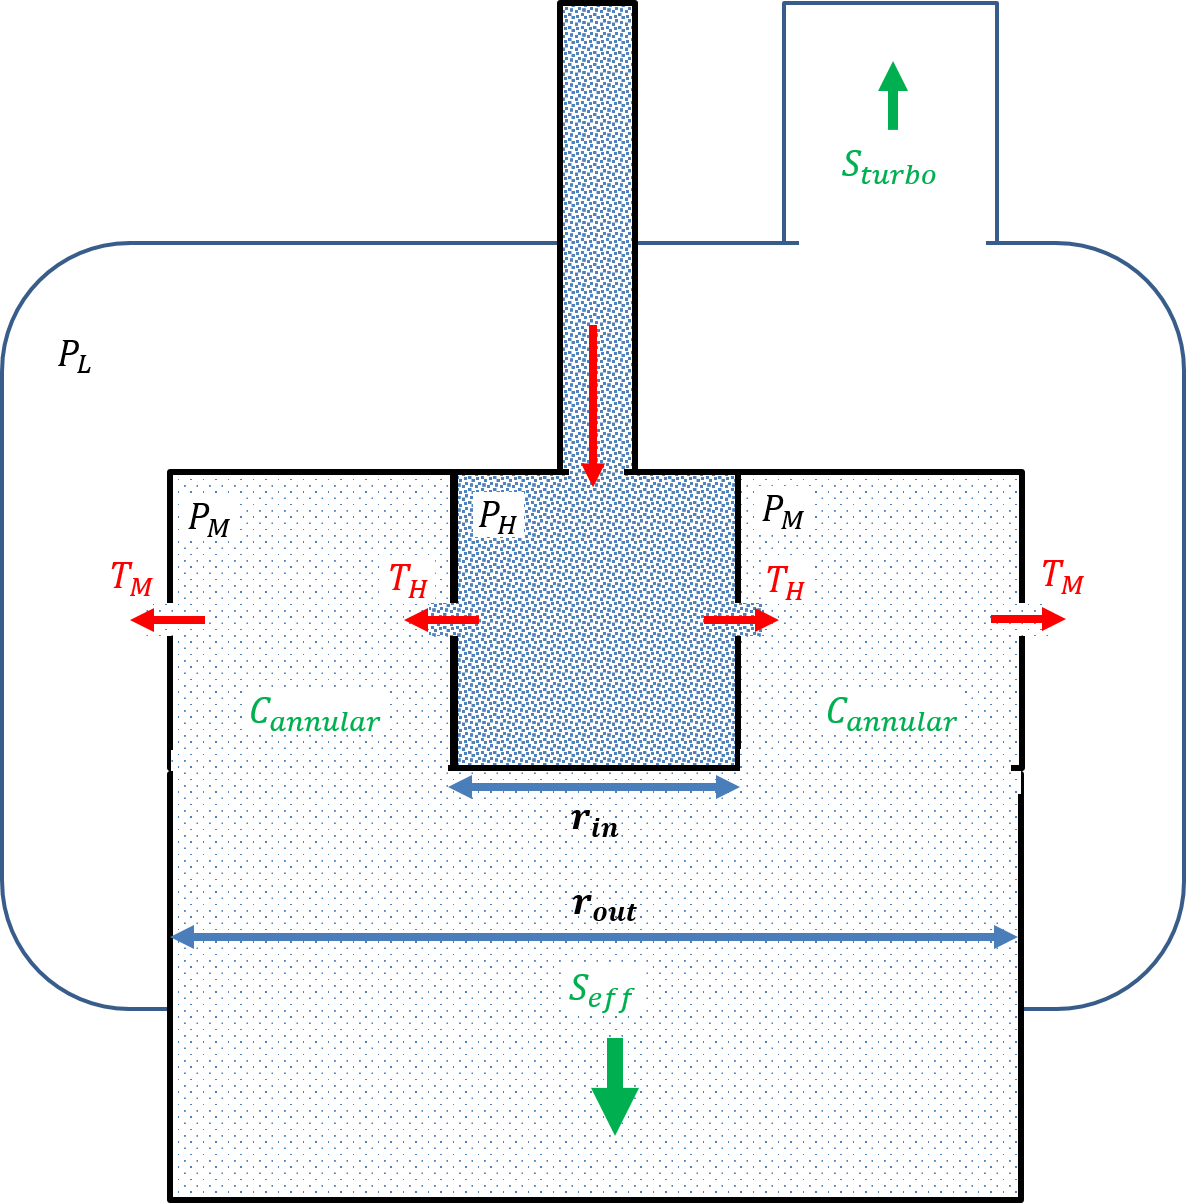
\includegraphics[width=0.9\textwidth]{figures/chap2/HPC_pressure_schematic.png}
	\caption{Schematic used to calculate the pressures inside the HPC and generation chamber. The dark blue region represents the inner pipe, the light blue region represents the outer pipe. Red arrows and text indicate gas sources, green arrows and text indicate flow towards the vacuum pumps; blue arrows and text indicate physical dimensions. $P_H$, $P_M$, and $P_L$ are the pressures of the inner pipe, outer pipe, and generation chamber, respectively; $S_{turbo}$, $S_{eff}$ and $C_{annular}$ are the turbo pumping speed, effective rough pumping speed and annular conductance, respectively; $T_H$ ($T_M$) is the gas throughput from the high (medium) pressure region into the medium (low) pressure region.}
	\label{fig:HPC_pressure_schematic}
\end{figure}

- why didn't you go with semi-infinite gas cell, or fiber-cell?

- basic design of high pressure cell

- limited pump speed $\rightarrow$ differential pumping is required

- gas load calculations (simple model)

harmonic yield results

advantages: much brighter due to pressure-length product. future application: can operate in low-pressure mode and reduce downstream generation gas contamination of target chamber.

disadvantages: difficult to align and initially install (once it's installed, alignment is easy). messed up mode. HHG instability at higher pressures.

\subsection{pulsed valve}

expensive

